\documentclass{article}
\PassOptionsToPackage{numbers,compress}{natbib}
\usepackage[main,final]{neurips_2026}
\makeatletter
\renewcommand{\@noticestring}{DSAA2011 Machine Learning, Course Project (Task A), HKUST(GZ), Fall 2026.}
\makeatother
\usepackage[utf8]{inputenc}
\usepackage[T1]{fontenc}
\usepackage{hyperref,url,booktabs,amsmath,amsfonts,graphicx,microtype,xcolor,placeins}
\graphicspath{{../figures/}}
\title{From Weather Snapshots to Seasonal Climate Signatures\\Recovering Australia's Climate Zones from Weather Observations}
\author{Group 7\\DSAA2011 (L02), HKUST(GZ)\\QIAO, Xiaolong \quad MO, Zijun \quad WANG, Zhifei \quad XIA, Youyue}
\newcommand{\DailyHGB}{0.659}
\newcommand{\DailyRF}{0.665}
\newcommand{\DailyAUC}{0.883}
\newcommand{\SeasonLR}{0.861}
\newcommand{\SeasonHGB}{0.807}
\newcommand{\SeasonLRAUC}{0.973}
\newcommand{\SeasonHGBAUC}{0.943}
\newcommand{\MatchedDaily}{0.759}
\newcommand{\SeasonGain}{0.047}
\newcommand{\MatchedLR}{0.702}
\newcommand{\SeasonLRGain}{0.159}
\newcommand{\SeasonFoldMean}{0.850}
\newcommand{\SeasonFoldSD}{0.085}
\newcommand{\SeasonFoldMin}{0.680}
\newcommand{\SeasonFoldMax}{0.975}
\newcommand{\SeasonBootLow}{0.760}
\newcommand{\SeasonBootHigh}{0.919}
\newcommand{\SeasonRows}{328}
\newcommand{\SeasonStations}{48}
\newcommand{\SeasonCoverage}{73.6\%}
\newcommand{\DailyTsnePurity}{0.631}
\newcommand{\DailyTsneTrust}{0.985}
\newcommand{\SeasonTsneSil}{0.112}
\newcommand{\DailyClusterARI}{0.098}
\newcommand{\SeasonClusterARI}{0.314}
\newcommand{\StationClusterARI}{0.345}
\newcommand{\DailyLR}{0.556}
\newcommand{\DailyDT}{0.577}
\newcommand{\DailyPoly}{0.654}
\newcommand{\HistoryHGB}{0.758}
\newcommand{\HistoryLR}{0.745}
\newcommand{\SpatialHGB}{0.565}
\newcommand{\CacheHits}{383}
\newcommand{\CacheMisses}{0}
\newcommand{\PythonVersion}{3.12.6}
\newcommand{\RunID}{f67d019ce7acf9e9}
\begin{document}
\maketitle

\begin{abstract}
We begin with a simple tension: climate is a long-run pattern, but each row in Rain in Australia describes only one day. We ask how much of an externally assigned five-zone climate label we can recover from weather when station identity and coordinates are withheld. We first keep the single-day experiment as a baseline. We then turn four 21-day windows around the equinoxes and solstices into one station-year seasonal signature. On the same station-held-out evaluation, daily HGB reaches macro-F1 \DailyHGB{}, while seasonal logistic regression reaches \SeasonLR{} with macro-AUC \SeasonLRAUC{}. A matched vote over four daily HGB predictions reaches \MatchedDaily{}, so the seasonal HGB signature gains \SeasonGain{} within the HGB classifier family (the difference uses unrounded scores); for LR, the corresponding gain is \SeasonLRGain{} within the LR family. Our evidence therefore supports temporal coverage as the more useful representation choice in this dataset, while the coverage filter, repeated years, four Tropical stations and one raster annotation limit the scope of the claim.
\end{abstract}

\section{Introduction}
We often speak about a place's weather and climate as if they were interchangeable. They are not. Climate is a recurring pattern of temperature, rainfall and atmospheric conditions, while a row in the supplied table is only one day's snapshot. A hot day can occur in several climate zones, and a cool day can occur in many others. We therefore ask a representation question: how much of an externally assigned climate-zone label can we recover from weather alone, and how does the answer change when we show the model more of the calendar?

The Australian data contain daily records from 49 named locations. We construct five project classes from an external Köppen--Geiger raster: Tropical, Arid, Subtropical, Mediterranean and Oceanic. The Mediterranean stations form separated geographic groups, which makes a purely positional story incomplete: distant places may share a seasonal weather pattern, while nearby places may differ. We do not use the map location to predict its own label. Instead, we compare a single-day weather snapshot with a compact description of the year's seasonal rhythm.

We follow the course tasks in one integrated pipeline. The daily analysis gives us a first impression of what weather states look like. Clustering then asks what structures appear without labels: first among individual days, then among longer station profiles. Finally, supervised models test whether the seasonal signature transfers to stations that were never used for training. Earlier exploratory work informed this design, but we present the final question and evidence as one continuous argument rather than as a sequence of disconnected experiment rounds.

\section{Data, labels and preprocessing}
The raw table has 145,460 rows and 49 locations. Norfolk Island is excluded because its raster assignment falls outside the five project groups, leaving 142,451 rows and 48 labelled stations. The class counts are unequal: Tropical has only four stations and Arid has seven. We therefore use pooled five-class macro-F1 as the headline metric and report station-balanced scores alongside it. A majority-class classifier would reach accuracy 0.322, which gives a useful but weak reference point.

We remove \texttt{Location}, future \texttt{RainTomorrow} and the unavailable \texttt{RISK\_MM} field from the predictors. We encode wind direction as circular vector components, retain wind speeds, transform rainfall as $\log(1+x)$, remove the redundant \texttt{RainToday} field, and encode day of year with sine and cosine. Median imputation and standardisation are learned inside each training-fold pipeline; histogram gradient boosting uses median imputation without scaling. The daily core contains 20 weather-derived columns. Station identifiers, labels and coordinates remain outside the feature matrix for grouping, diagnostics and target construction.

Our main representation uses four 21-day windows centred on March 20, June 21, September 22 and December 21. Each window contributes means and standard deviations for weather variables, rainy-day fraction and temperature-range summaries. We keep a station-year only when every window has at least seven valid days. This produces \SeasonRows{} station-year signatures from \SeasonStations{} stations, with mean complete coverage \SeasonCoverage{}. No station ID, coordinate or target label enters these features. The four dates are a transparent proxy for an annual weather pattern; they are not a new climate ground truth.

\section{Mandatory tasks}
\subsection{Daily t-SNE visualization}
For the required visualization, we sample 1,200 daily rows per class, impute and standardise the 20-dimensional core, and fit t-SNE with perplexity 30. We balance the sample so the four Tropical stations are visible rather than overwhelmed by the larger classes; the labels do not optimize the embedding. The t-SNE trustworthiness is \DailyTsneTrust{} and a diagnostic 10-neighbour zone purity is \DailyTsnePurity{}. These are descriptive local-neighbourhood measures, not held-out prediction scores: days from the same station appear on both sides of the diagnostic neighbourhood folds.

\begin{figure}[t]\centering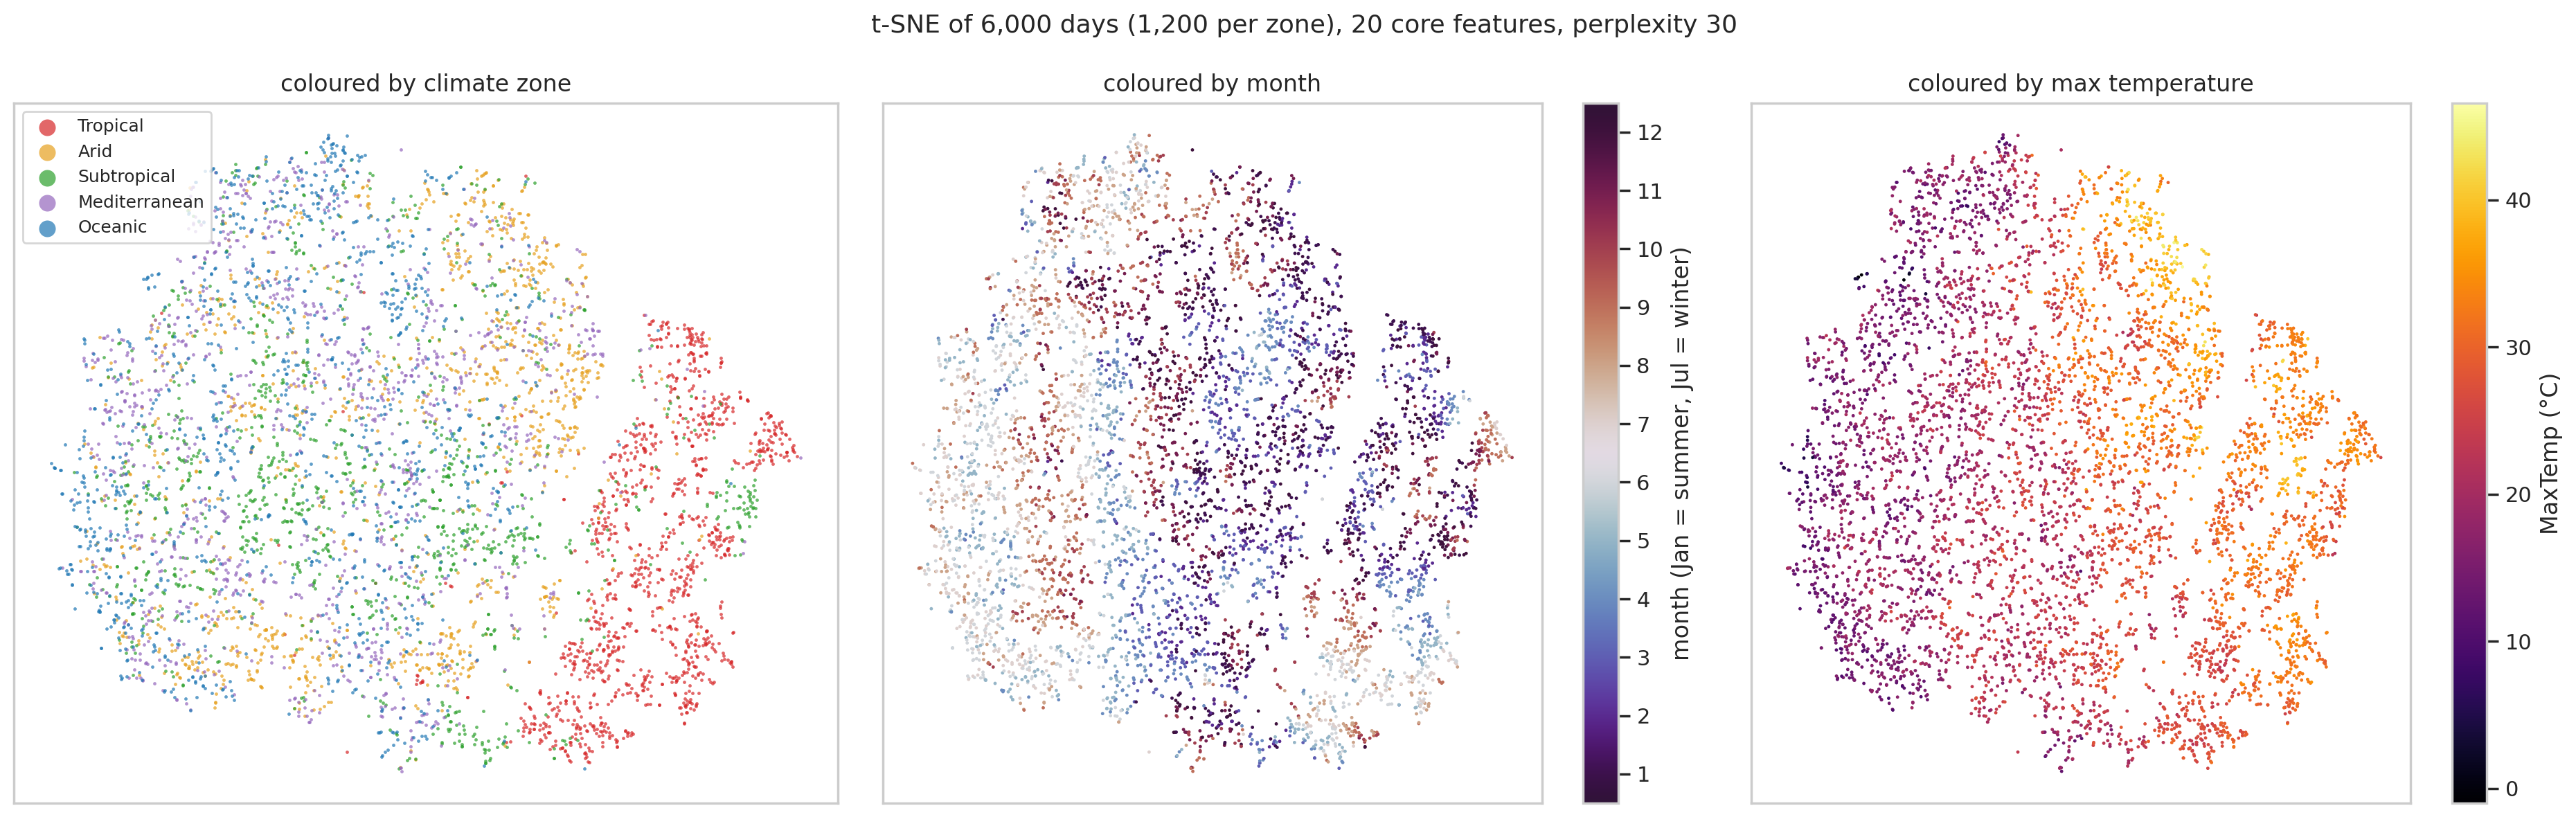
\includegraphics[width=\linewidth]{p2_tsne_main}
\caption{Daily weather snapshot t-SNE, coloured by the five external climate groups. The plot motivates treating a day as a baseline rather than a complete climate description.}\label{fig:dailytsne}
\end{figure}

\subsection{Clustering: from weather states to station profiles}
Clustering answers a different question from prediction. We do not ask it to maximize agreement with the climate labels. We ask what repeatable structures the weather itself creates, and whether those structures become more climate-like after temporal aggregation.

\paragraph{Single days form shared weather states.}
We fit K-means, Ward agglomeration and a full-covariance Gaussian mixture to the same balanced daily sample. For $k=2,\ldots,10$ we record silhouette, Davies--Bouldin, Calinski--Harabasz, stability and external ARI. We select a descriptive daily partition using a stability threshold and the average rank of the three internal compactness measures; the external label scores are reserved for interpretation. The selected K-means solution has $k=3$, but its silhouette is modest. This is a stable partition of overlapping weather geometry, not evidence of three sharply separated physical regimes.

The three clusters are nevertheless interpretable. One is warm, with mean maximum temperature 30.6 degrees C. The other two have almost the same maximum temperature, 18.9 and 19.1 degrees C, but separate through pressure and wind: one is higher-pressure with weaker wind, while the other is lower-pressure with stronger wind and a higher transformed-rainfall mean. Only 40\% of the warm cluster is Tropical in the deliberately balanced sample. The low daily ARI of \DailyClusterARI{} therefore tells us something useful: a day can resemble the weather of several climate zones.

\begin{figure}[t]\centering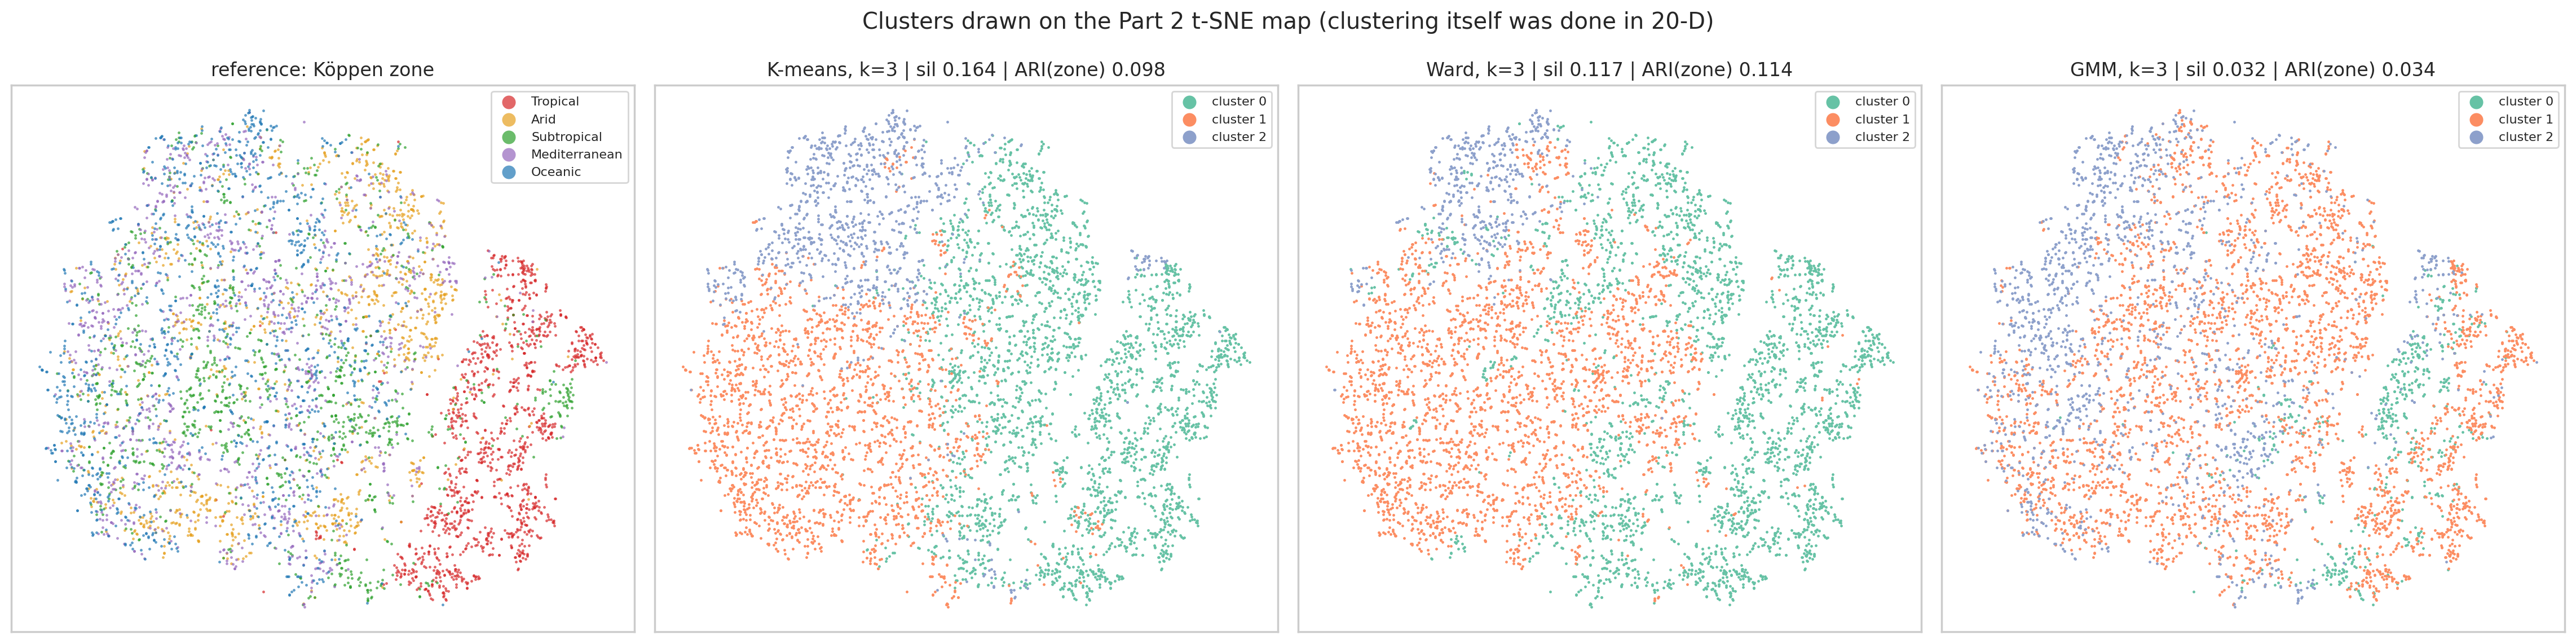
\includegraphics[width=0.98\linewidth]{p3_clusters_on_tsne}
\caption{Daily clusters shown on the same t-SNE coordinates as the climate reference. Clustering was fitted in the original 20-dimensional feature space; t-SNE is only a display. The broad warm region is visible, while climate colours and weather-cluster colours remain mixed.}\label{fig:dailyclusters}
\end{figure}

\paragraph{Monthly station profiles reveal the bridge to climate.}
To see what temporal aggregation changes, we also construct a descriptive profile for each of the 48 stations: twelve monthly means of maximum temperature, minimum temperature, afternoon humidity and rainfall. We standardise these 48 features and apply Ward clustering. At $k=5$, the map has ARI \StationClusterARI{} with the external labels. This is not a controlled improvement over daily clustering because the unit, variables and clustering rule all change. Its value is interpretive. The four Tropical stations form one cluster; nine east-coast Subtropical stations form another; and some distant southwest and southeast stations share a cluster. The same weather profile can therefore recur across geographic distance, although the clusters still mix Mediterranean and Oceanic labels.

\begin{figure}[t]\centering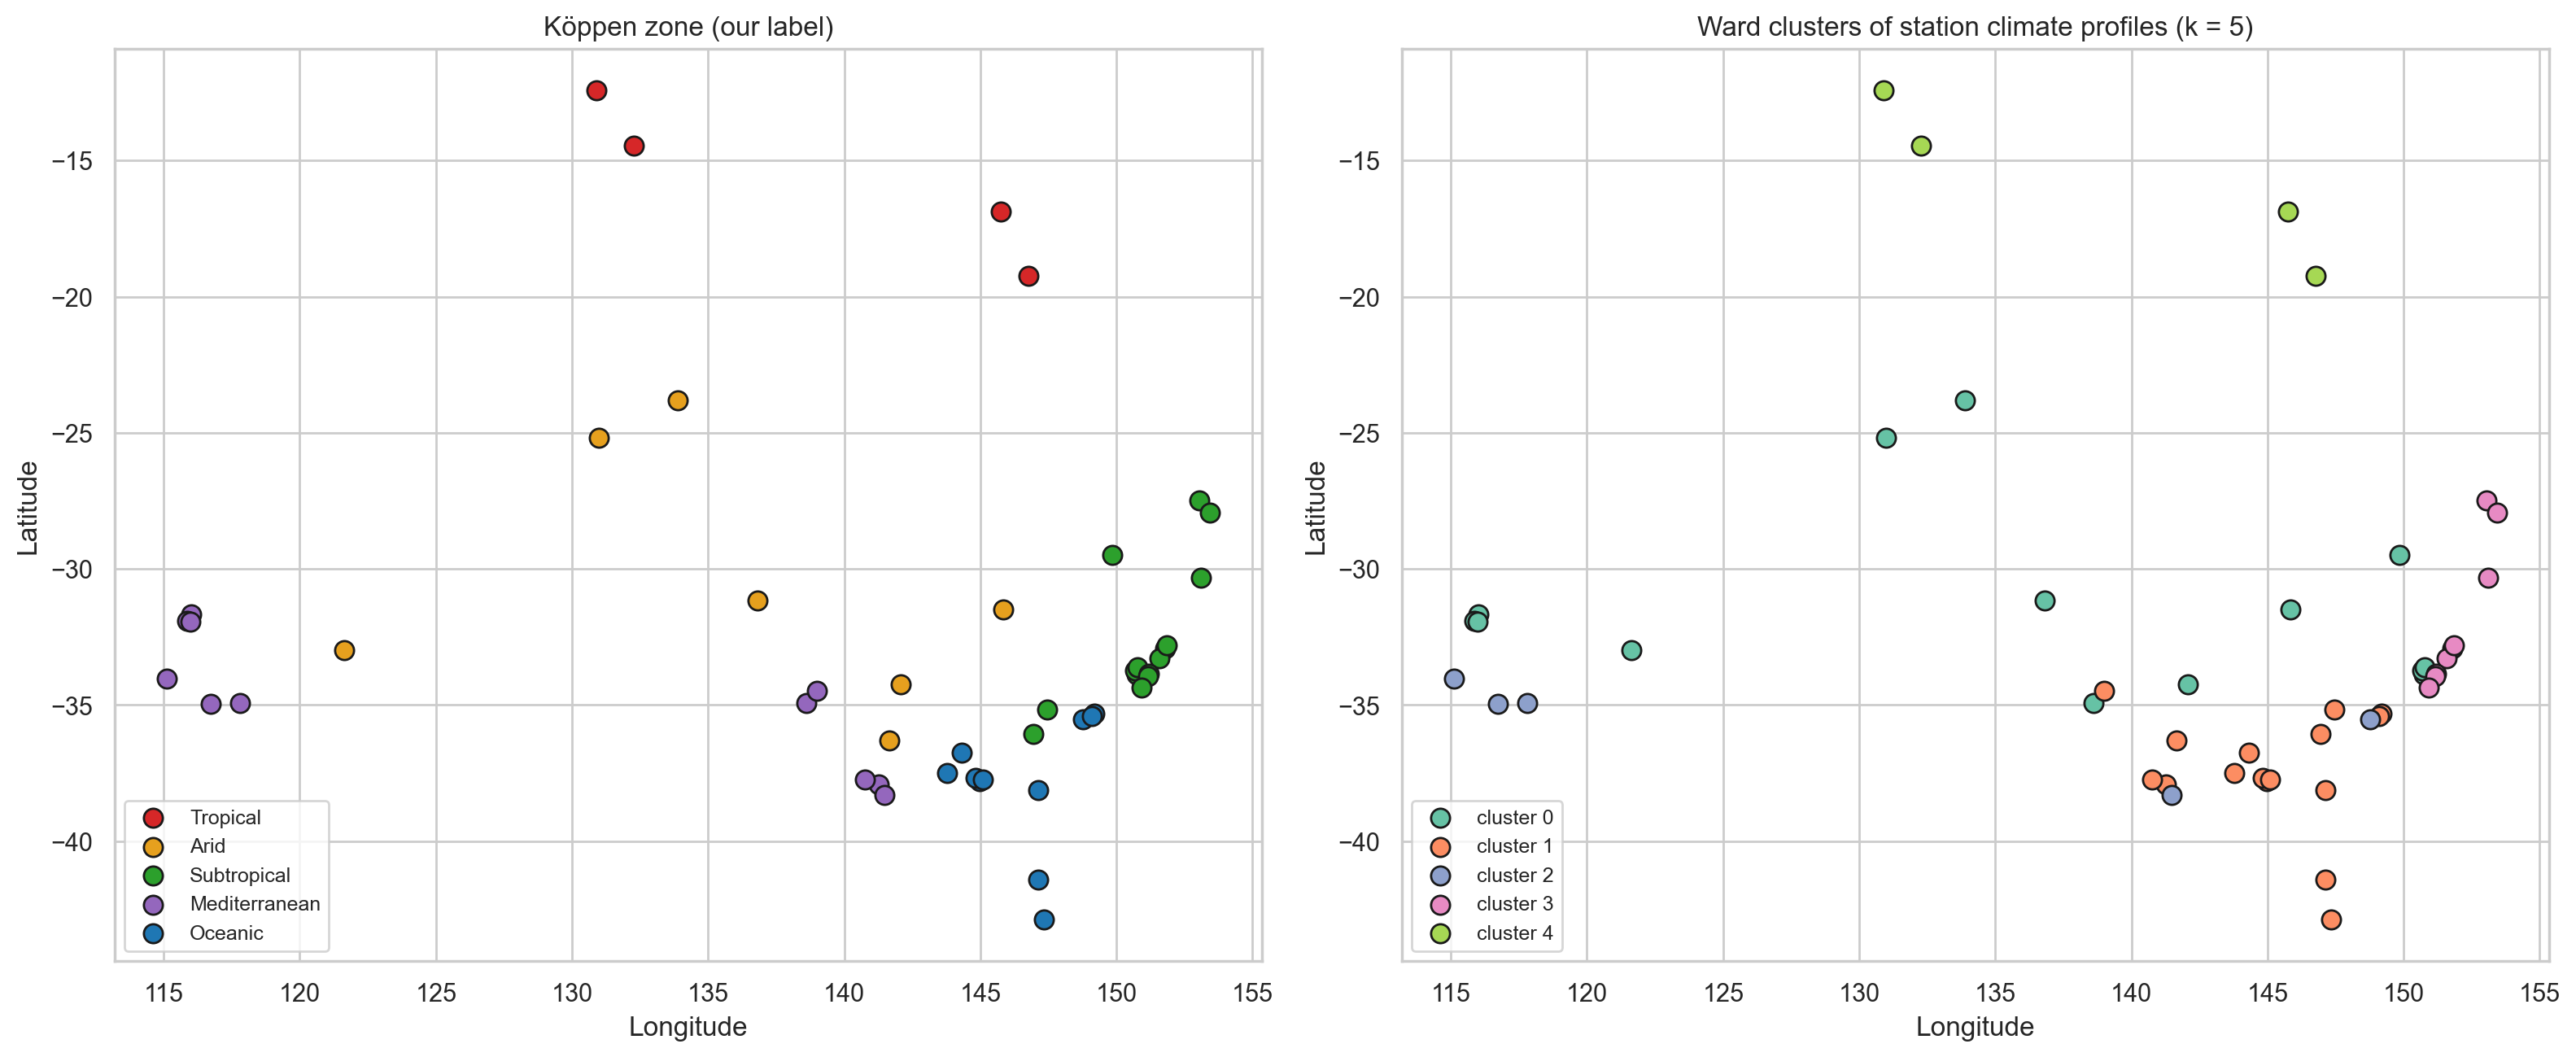
\includegraphics[width=0.92\linewidth]{p3_station_clusters_map}
\caption{Köppen labels and Ward clusters of 48 station-level monthly weather profiles. Coordinates are excluded from clustering and used only to plot the station locations. The five-cluster partition is a reference comparison chosen for interpretation, not an internally selected optimum.}\label{fig:stationclusters}
\end{figure}

\paragraph{Seasonal signatures do not naturally fall into five climate zones.}
We repeat a smaller K-means and Ward sweep on the four-season station-year signatures. Internal compactness measures prefer $k=2$, while the largest external ARI occurs at $k=7$. The latter is reported only as a post-hoc description after looking at the labels; it is not an unsupervised discovery of seven climate zones. The comparison is valuable precisely because it separates two ideas: natural weather geometry can be stable or compact without matching a categorical climate map, while a supervised classifier can still combine many weak seasonal signals.

\begin{table}[t]
\centering
\small
\setlength{\tabcolsep}{2pt}
\caption{Daily and seasonal clustering comparisons. Daily K-means $k=3$ is chosen by an internal-metric and stability rule. Seasonal internal metrics prefer $k=2$; the ARI-maximising $k=7$ row is a post-hoc label comparison.}\label{tab:cluster}
\begin{tabular}{lrrrrrr}\toprule
Algorithm & Daily sil. & Daily ARI & Season $k$ (sil.) & Season sil. & Post-hoc $k$ & Post-hoc ARI \\ \midrule
K-means & 0.164 & 0.098 & 2 & 0.254 & 7 & 0.314 \\
Ward & 0.117 & 0.114 & 2 & 0.290 & 7 & 0.282 \\
\bottomrule
\end{tabular}
\end{table}
\begin{figure}[t]\centering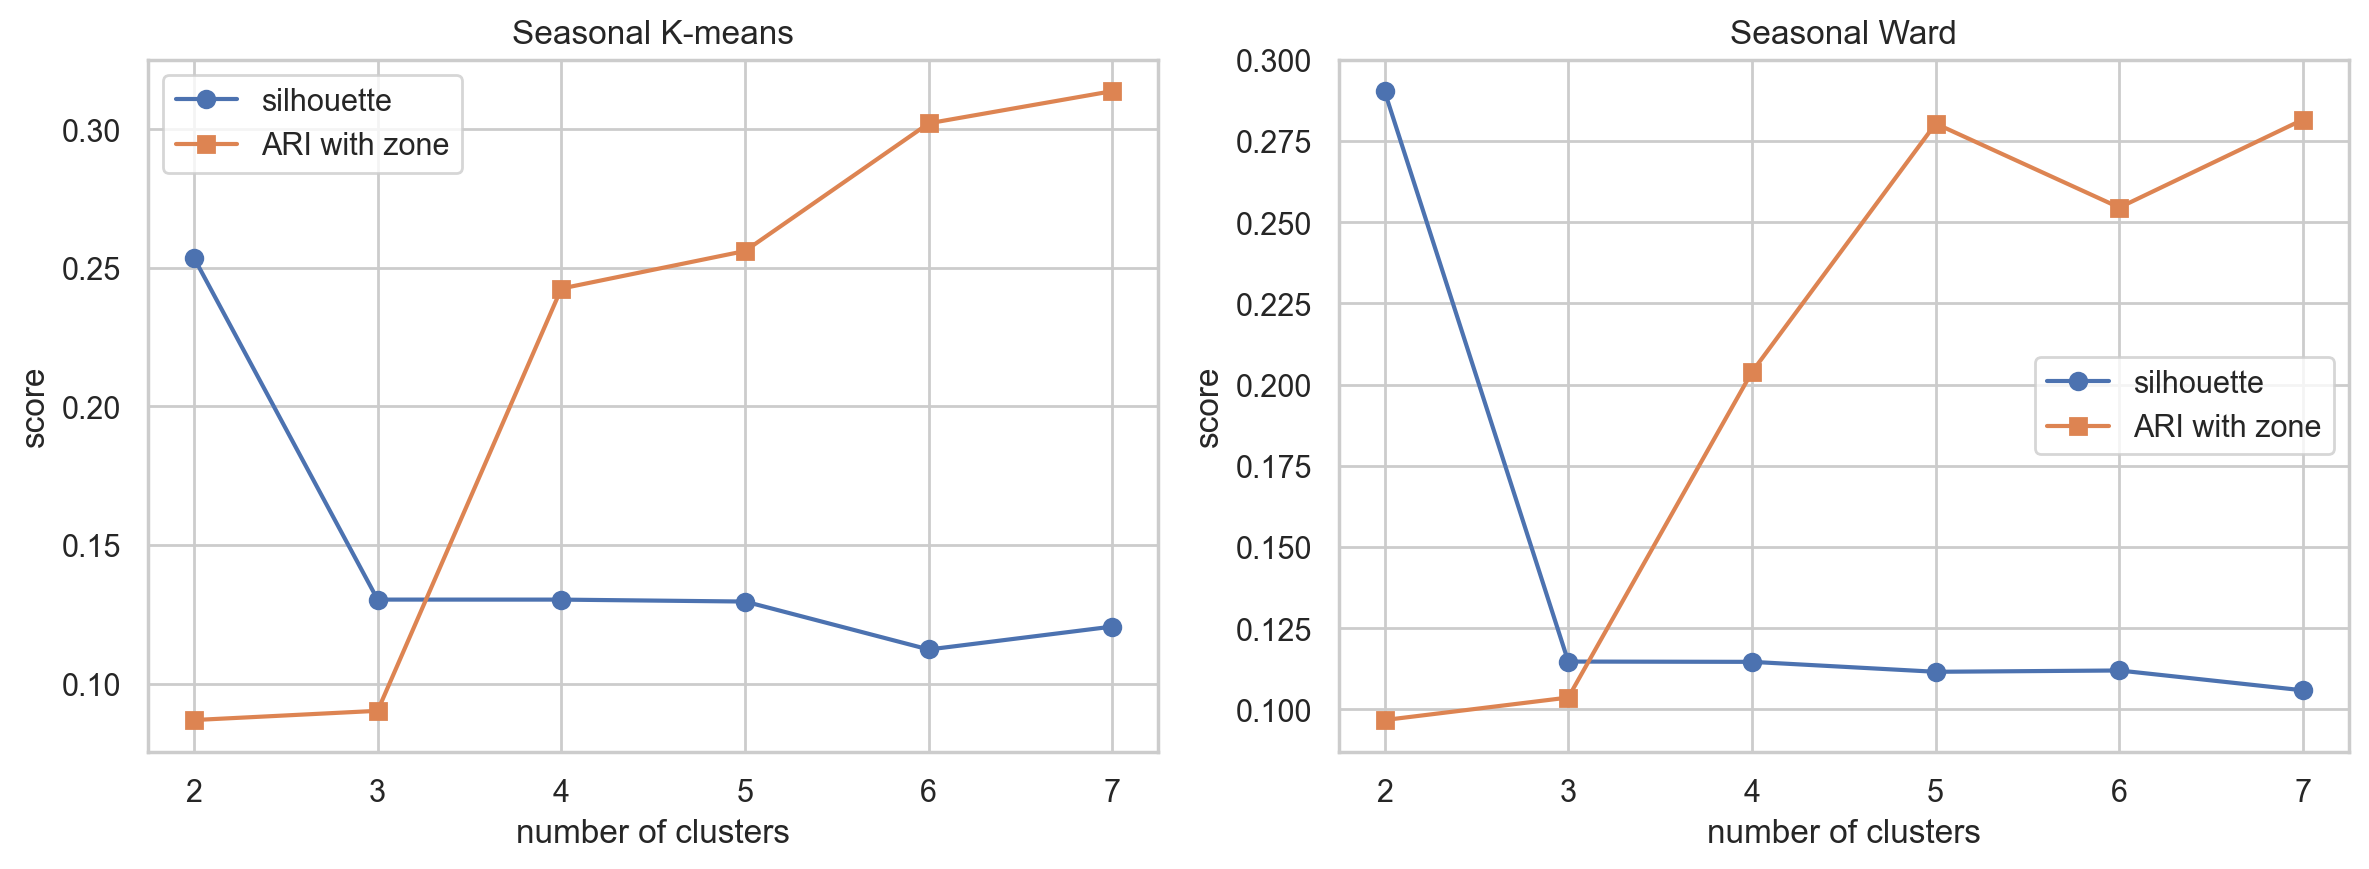
\includegraphics[width=\linewidth]{p7_seasonal_clustering}
\caption{Seasonal clustering sweep. Internal metrics favour $k=2$; the ARI-maximising $k=7$ result is a post-hoc label comparison and is not used as an unsupervised model-selection claim.}\label{fig:seasoncluster}
\end{figure}

\subsection{Prediction and required evaluation}
We treat the course-style random split as a required diagnostic and the station-held-out split as the main transfer test. The required models are multinomial logistic regression (LR) and a default decision tree (DT). We report accuracy and macro-F1 on the train, test and entire sets, then evaluate additional models under outer folds that hold out whole stations. The random split is intentionally easier because the same locations occur on both sides. Tuned LR and DT, random forest, histogram gradient boosting and polynomial LR provide the open-ended model comparison; all preprocessing and probability estimates stay inside the fitting pipeline.

\begin{table}[t]
\centering
\small
\setlength{\tabcolsep}{4pt}
\caption{Required train/test/entire metrics under the course-style random split.}\label{tab:required}
\begin{tabular}{llrrr}\toprule
Model & Set & Accuracy & Macro-F1 & Weighted-F1 \\ \midrule
LR & train & 0.604 & 0.620 & 0.598 \\
LR & test & 0.599 & 0.615 & 0.593 \\
LR & entire & 0.602 & 0.618 & 0.597 \\
DT & train & 1.000 & 1.000 & 1.000 \\
DT & test & 0.652 & 0.669 & 0.652 \\
DT & entire & 0.895 & 0.900 & 0.896 \\
\bottomrule
\end{tabular}
\end{table}
\begin{figure}[t]\centering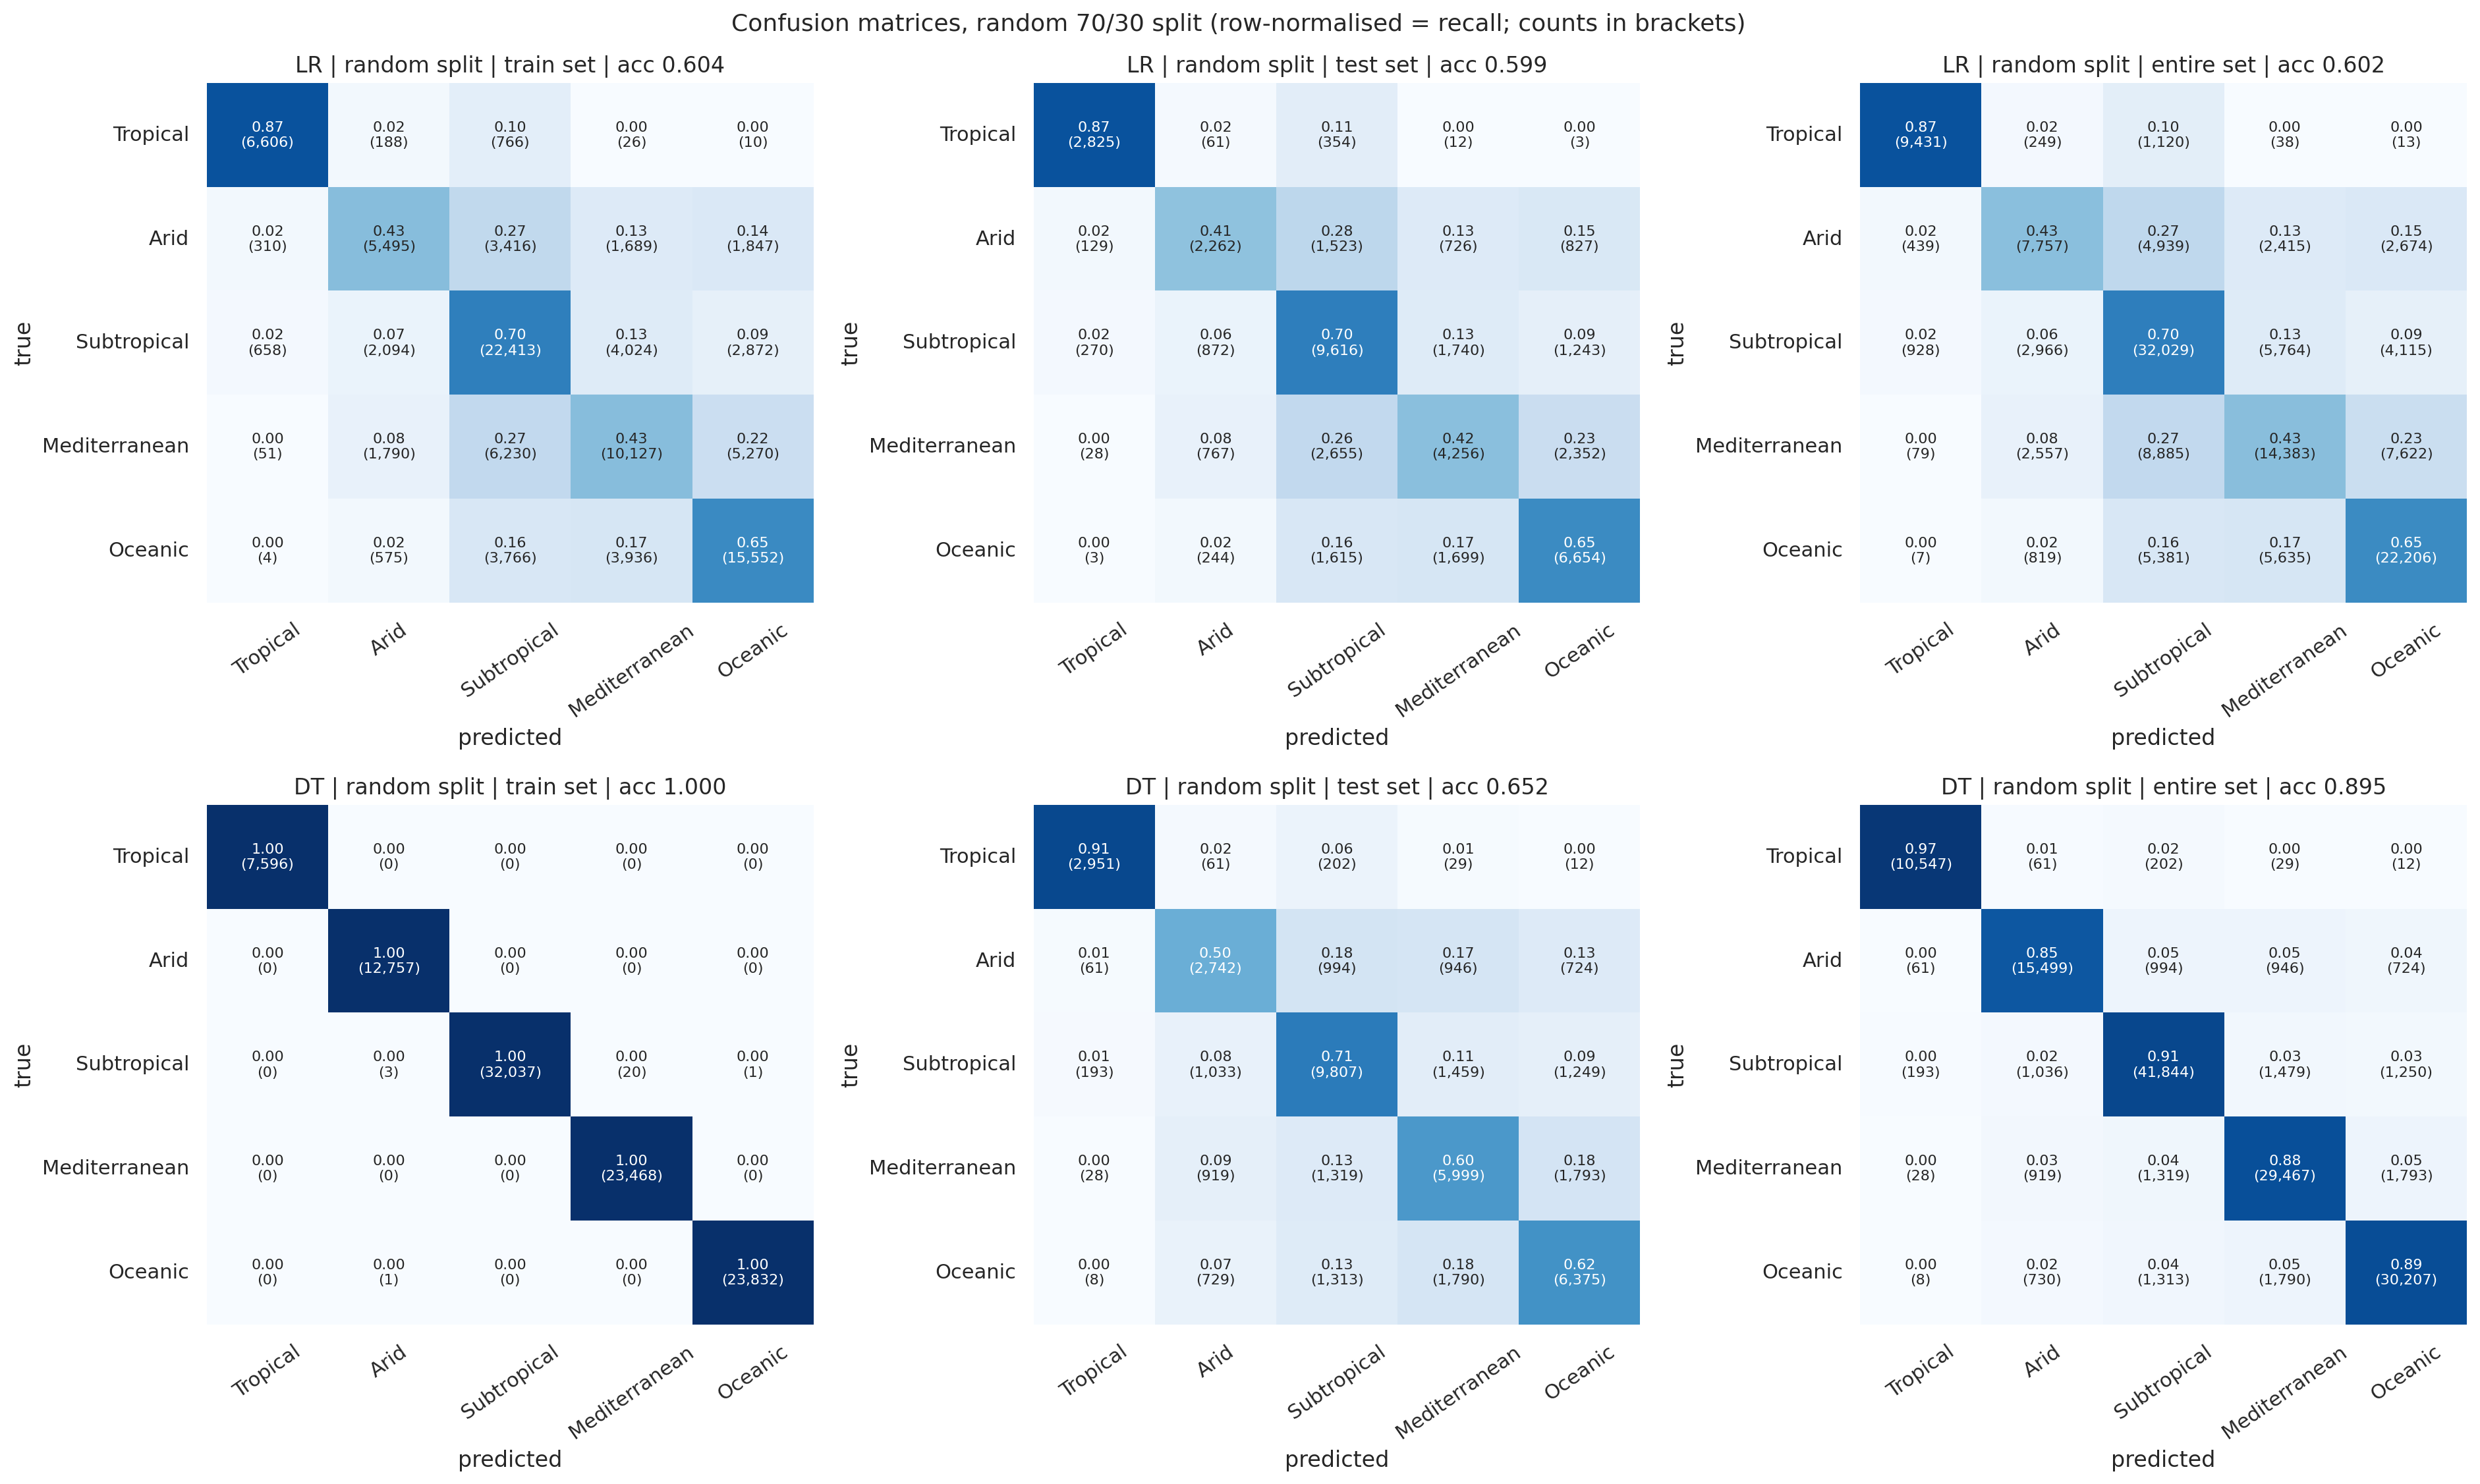
\includegraphics[width=0.98\linewidth]{p4_confusion_random}
\caption{Required random-split confusion matrices for LR and the default decision tree, including train, test and entire-set panels. The entire-set panels are descriptive because the model was fitted on the random training subset.}\label{fig:requiredcm}
\end{figure}
\begin{figure}[t]\centering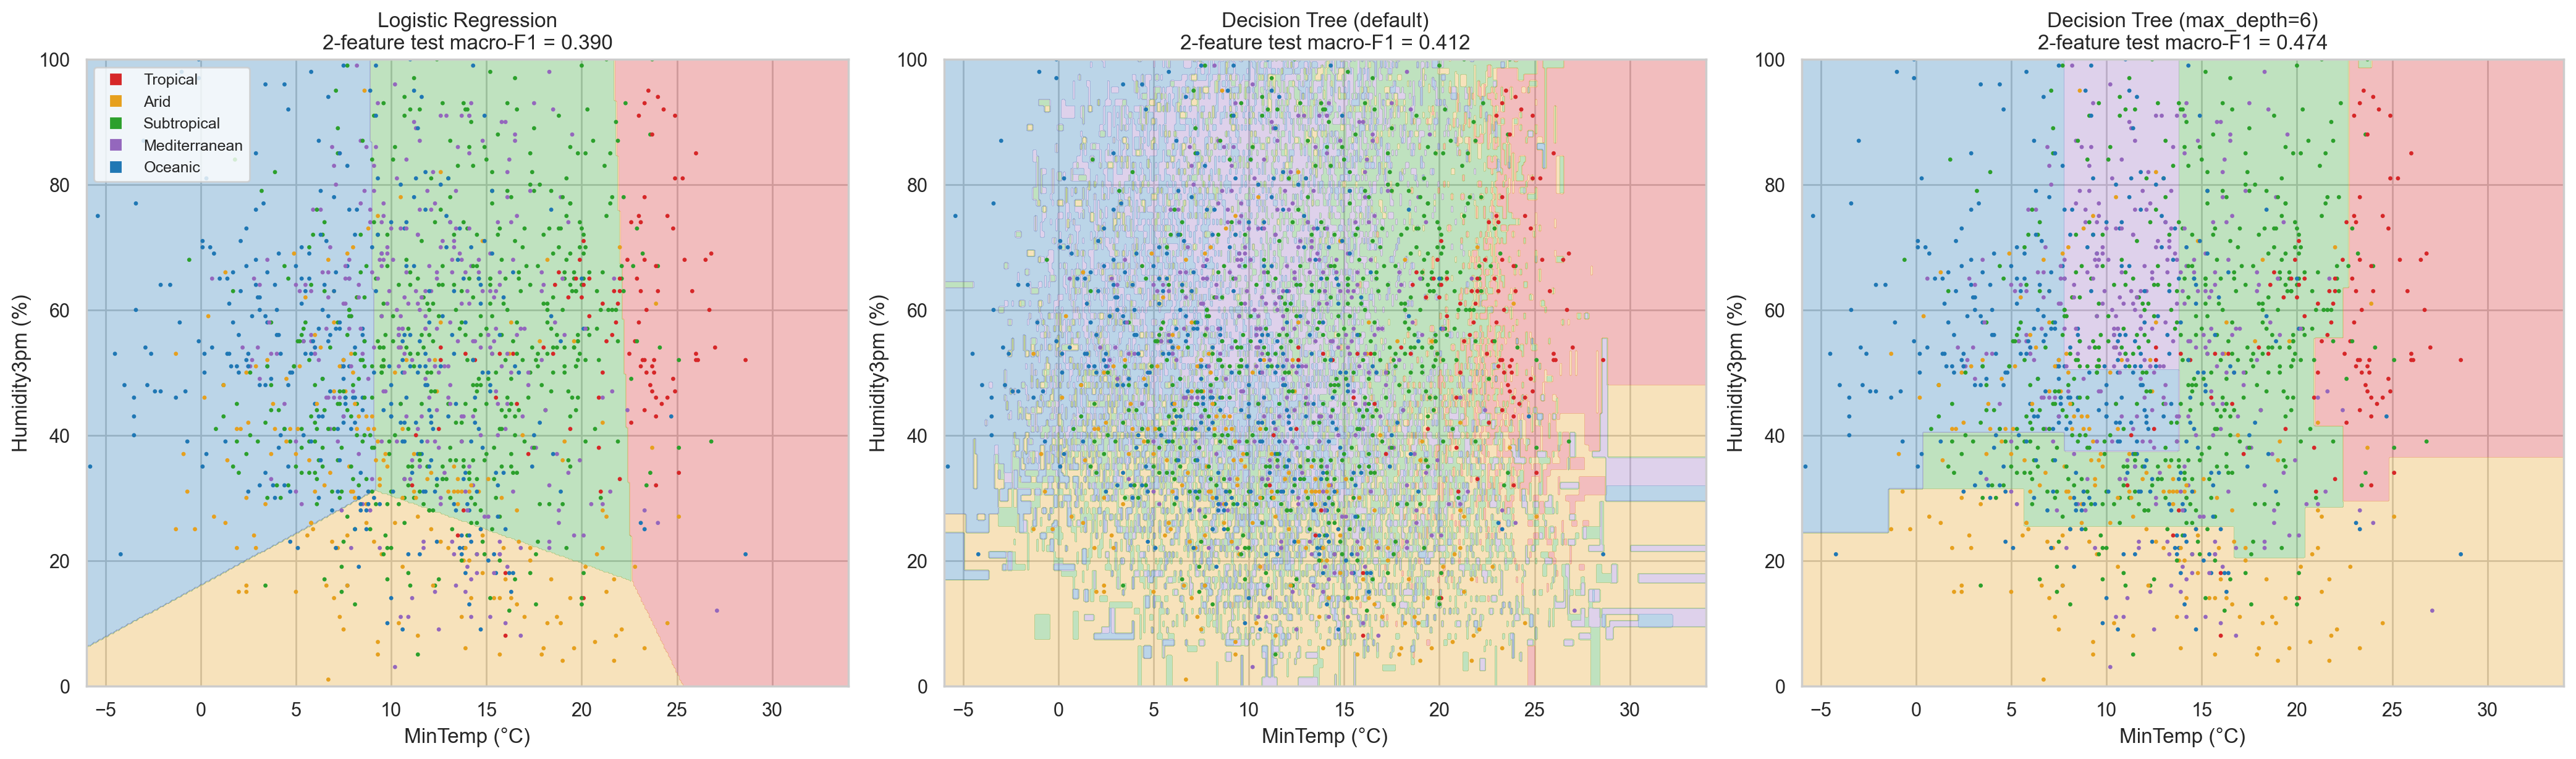
\includegraphics[width=0.98\linewidth]{p4_decision_boundary}
\caption{Required two-feature decision-boundary illustration for the daily baseline. It is a low-dimensional visual diagnostic, not the full-feature model used for the headline scores.}\label{fig:boundary}
\end{figure}

\begin{table}[t]
\centering
\small
\setlength{\tabcolsep}{4pt}
\caption{Daily weather baseline and model comparison. Primary is pooled station-held-out macro-F1; seed range reuses the same station network.}\label{tab:daily}
\begin{tabular}{lrrrrr}\toprule
Model & Primary F1 & Seed mean & Seed range & Station-bal. & AUC \\ \midrule
LR & 0.556 & 0.549 & 0.538--0.556 & 0.556 & 0.823 \\
DT-tuned & 0.577 & 0.569 & 0.553--0.577 & 0.577 & 0.812 \\
RF & 0.665 & 0.651 & 0.633--0.665 & 0.665 & 0.886 \\
HGB & 0.659 & 0.647 & 0.632--0.659 & 0.657 & 0.883 \\
HGB-tuned & 0.660 & 0.646 & 0.629--0.660 & 0.658 & 0.883 \\
PolyLR & 0.654 & 0.642 & 0.621--0.654 & 0.654 & 0.878 \\
\bottomrule
\end{tabular}
\end{table}
\begin{figure}[t]\centering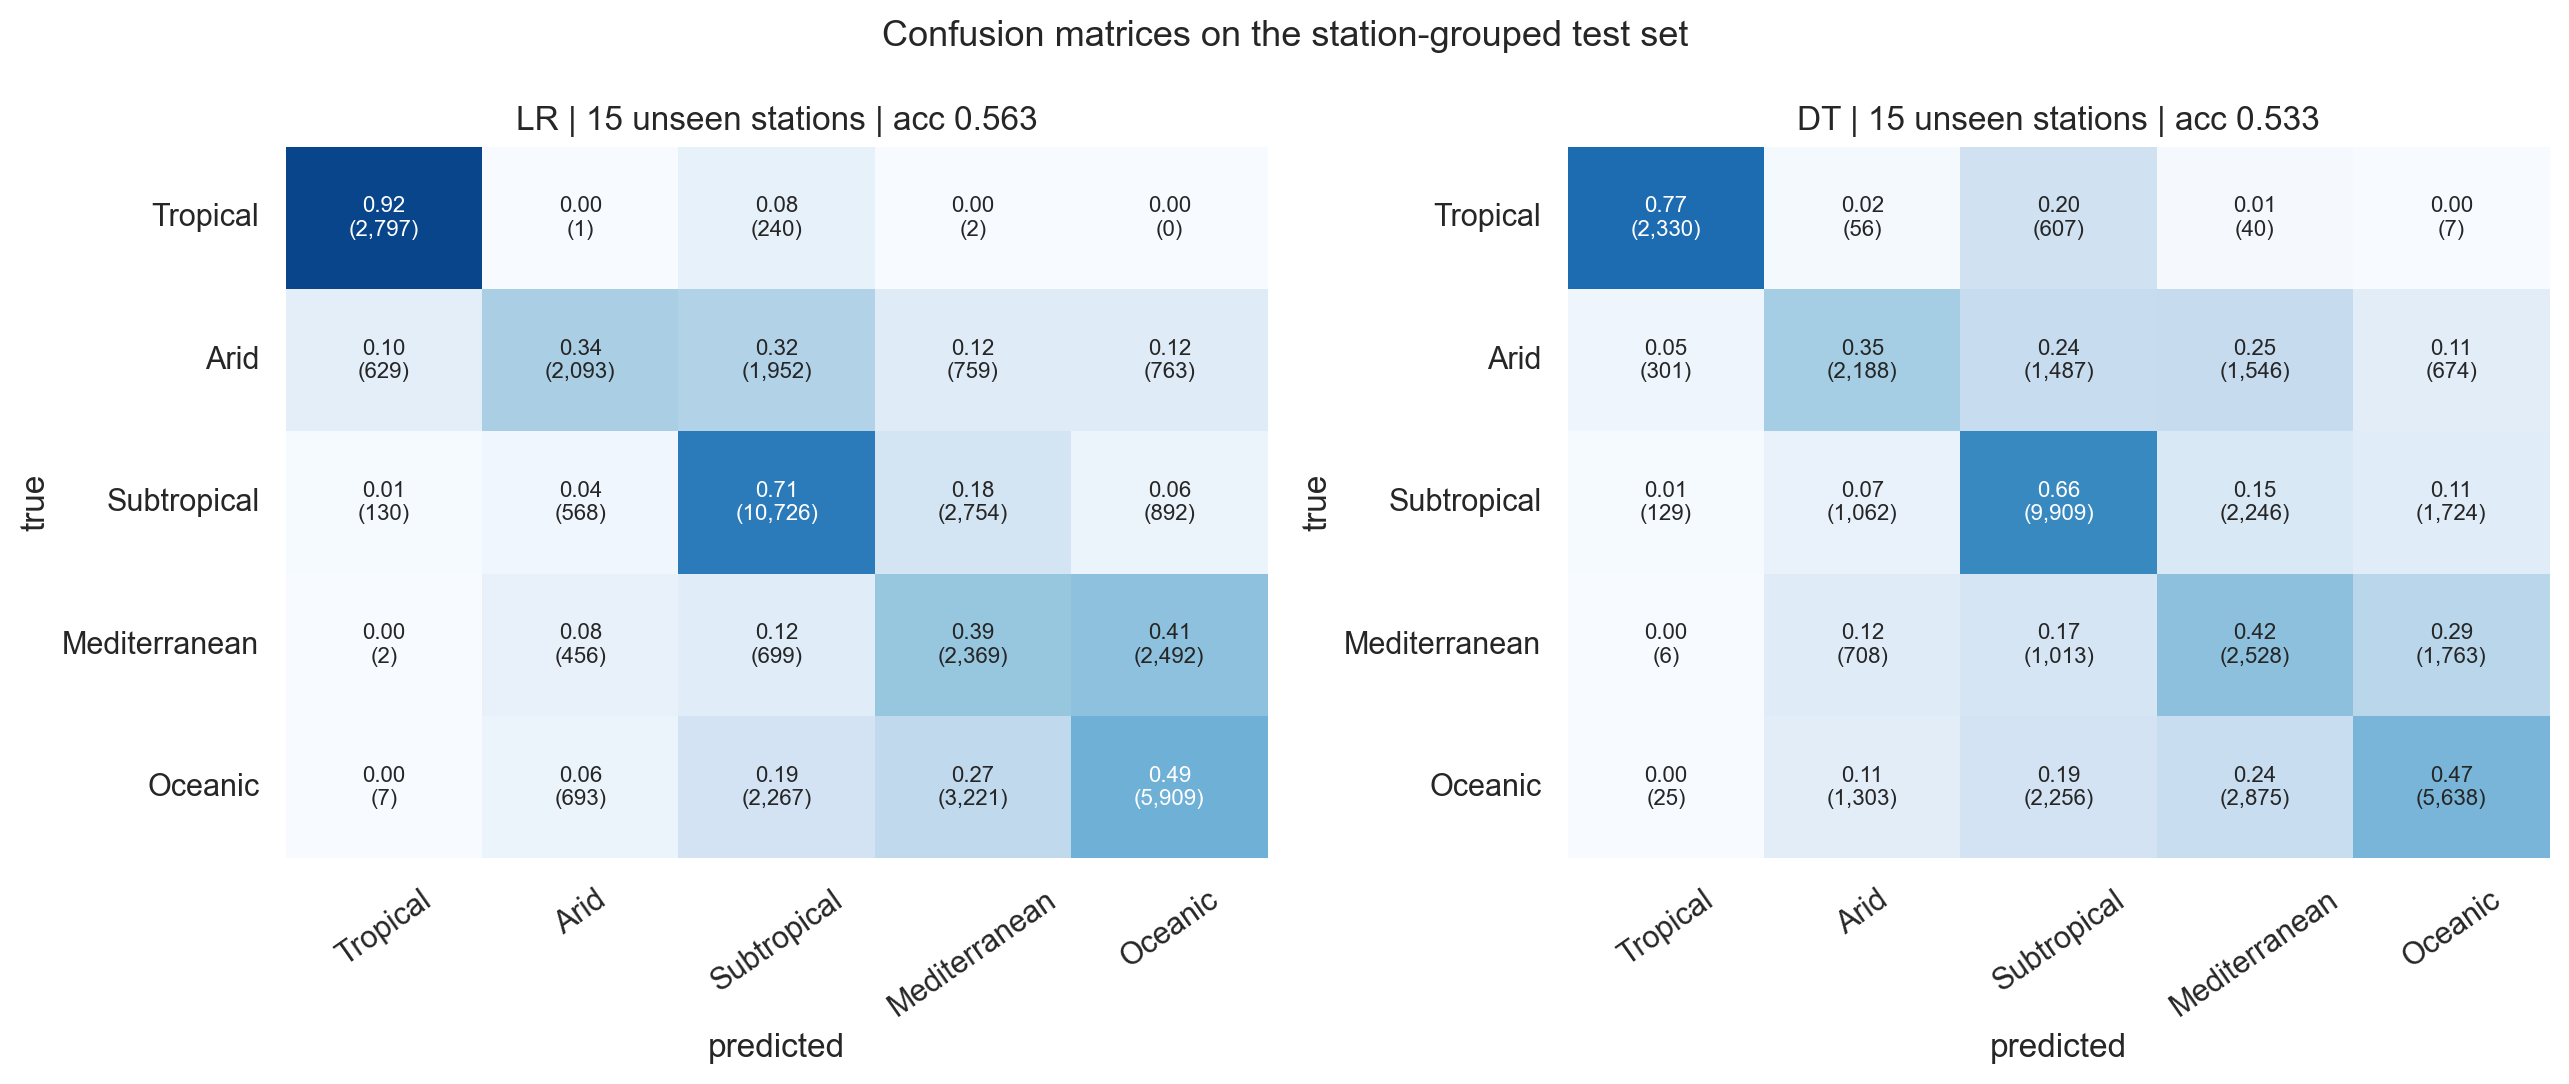
\includegraphics[width=\linewidth]{p4_confusion_grouped}
\caption{Station-held-out confusion matrix for the daily baseline. Rows are true zones and columns are predictions; the uneven class support is why macro metrics accompany accuracy.}\label{fig:dailycm}
\end{figure}

We compute precision, recall, F1, confusion matrices and one-vs-rest ROC/AUC from the same predictions. The daily HGB macro-AUC is \DailyAUC{}. Under the random split, the default tree fits the training rows perfectly but drops on the test rows; its entire-set score is therefore not a separate generalisation estimate. The grouped column in the following validation table is the relevant transfer check because every outer test station is unseen during fitting and tuning.

\begin{table}[t]
\centering
\small
\setlength{\tabcolsep}{4pt}
\caption{Held-out results after inner-fold hyperparameter selection; tuning never uses the outer test stations.}\label{tab:validation}
\begin{tabular}{lrrrr}\toprule
Model & Random F1 & Grouped F1 & Random AUC & Grouped AUC \\ \midrule
LR-tuned & 0.615 & 0.554 & 0.859 & 0.821 \\
DT-tuned & 0.691 & 0.558 & 0.889 & 0.809 \\
\bottomrule
\end{tabular}
\end{table}

Our daily history analysis uses station-disjoint inner folds to compare trailing windows. The selected-window scores are LR \HistoryLR{} and HGB \HistoryHGB{} macro-F1. These are selected-procedure estimates, not scores chosen from the outer test folds. The required metric discussion is:

{\small\emph{The daily weather baseline contains real but limited climate information. Under the station-held-out protocol, HGB reaches 0.659 macro-F1 and 0.883 macro-AUC, while LR reaches 0.556. The random row split is easier because the same stations occur on both sides, so it is not used as the headline estimate. The required train/test/entire-set tables show the default tree's large fit gap, whereas LR has a smaller gap. Precision, recall and F1 remain uneven: Arid and Mediterranean sites are confused most often. The four-season signature changes the unit to station-year and retains only 73.6\% of candidate years, but seasonal LR reaches 0.861 macro-F1 and 0.973 macro-AUC on held-out stations. This supports the motivation that temporal coverage matters, while the coverage filter, station-year dependence and one external label map limit how broadly the result can be generalised.}}

\begin{figure}[t]\centering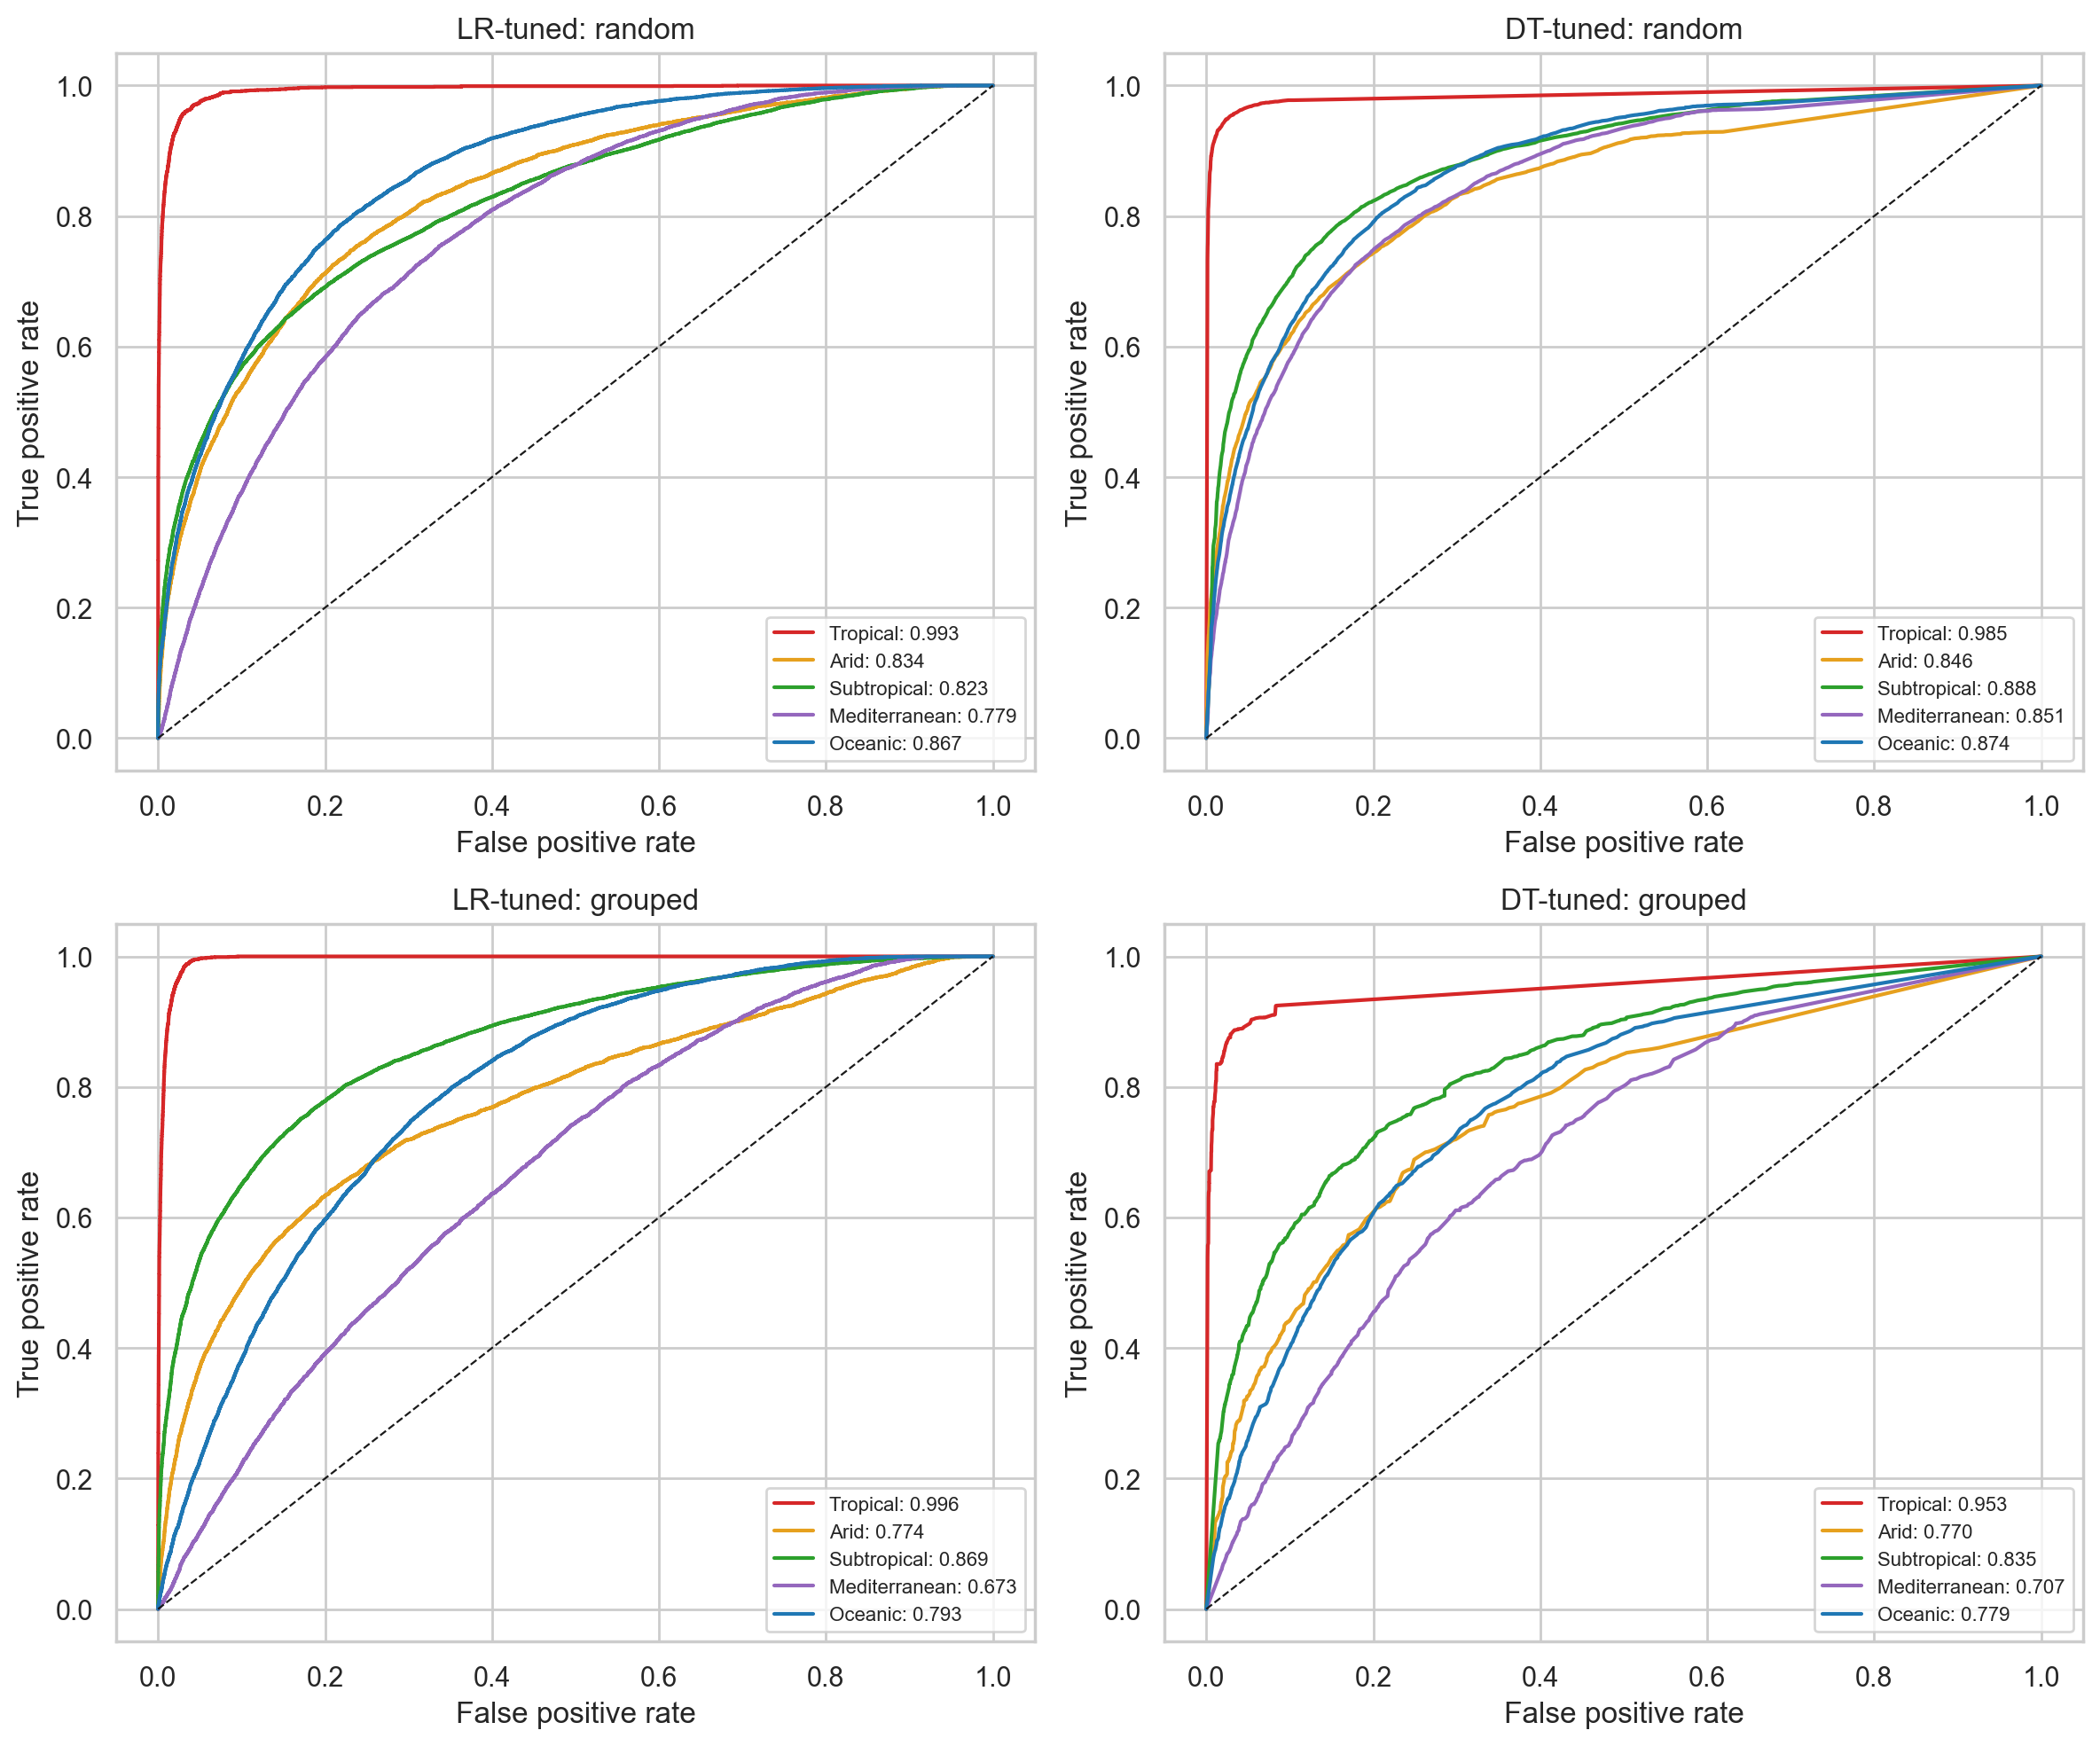
\includegraphics[width=\linewidth]{p5_roc_tuned}
\caption{ROC curves for the simple tuned classifiers on the course holdouts. Primary conclusions use station-held-out out-of-fold predictions.}\label{fig:roc}
\end{figure}

\section{Open-ended exploration: seasonal signatures}
\subsection{Four windows and coverage}
The central open-ended experiment turns multiple weather observations into one station-year row. We use means to describe seasonal state, standard deviations to retain variability, rainy-day fractions to preserve event frequency, and temperature ranges to represent within-window contrast. We report coverage before fitting so that the retained population is explicit rather than hidden inside the final score.

\begin{table}[t]
\centering
\small
\setlength{\tabcolsep}{4pt}
\caption{Coverage of complete four-window station-year signatures; at least seven valid days are required in every window.}\label{tab:coverage}
\begin{tabular}{lrrr}\toprule
Zone & Complete & Candidate & Coverage \\ \midrule
Tropical & 25 & 35 & 0.714 \\
Arid & 42 & 56 & 0.750 \\
Subtropical & 106 & 142 & 0.746 \\
Mediterranean & 77 & 103 & 0.748 \\
Oceanic & 78 & 108 & 0.722 \\
\bottomrule
\end{tabular}
\end{table}
\begin{figure}[t]\centering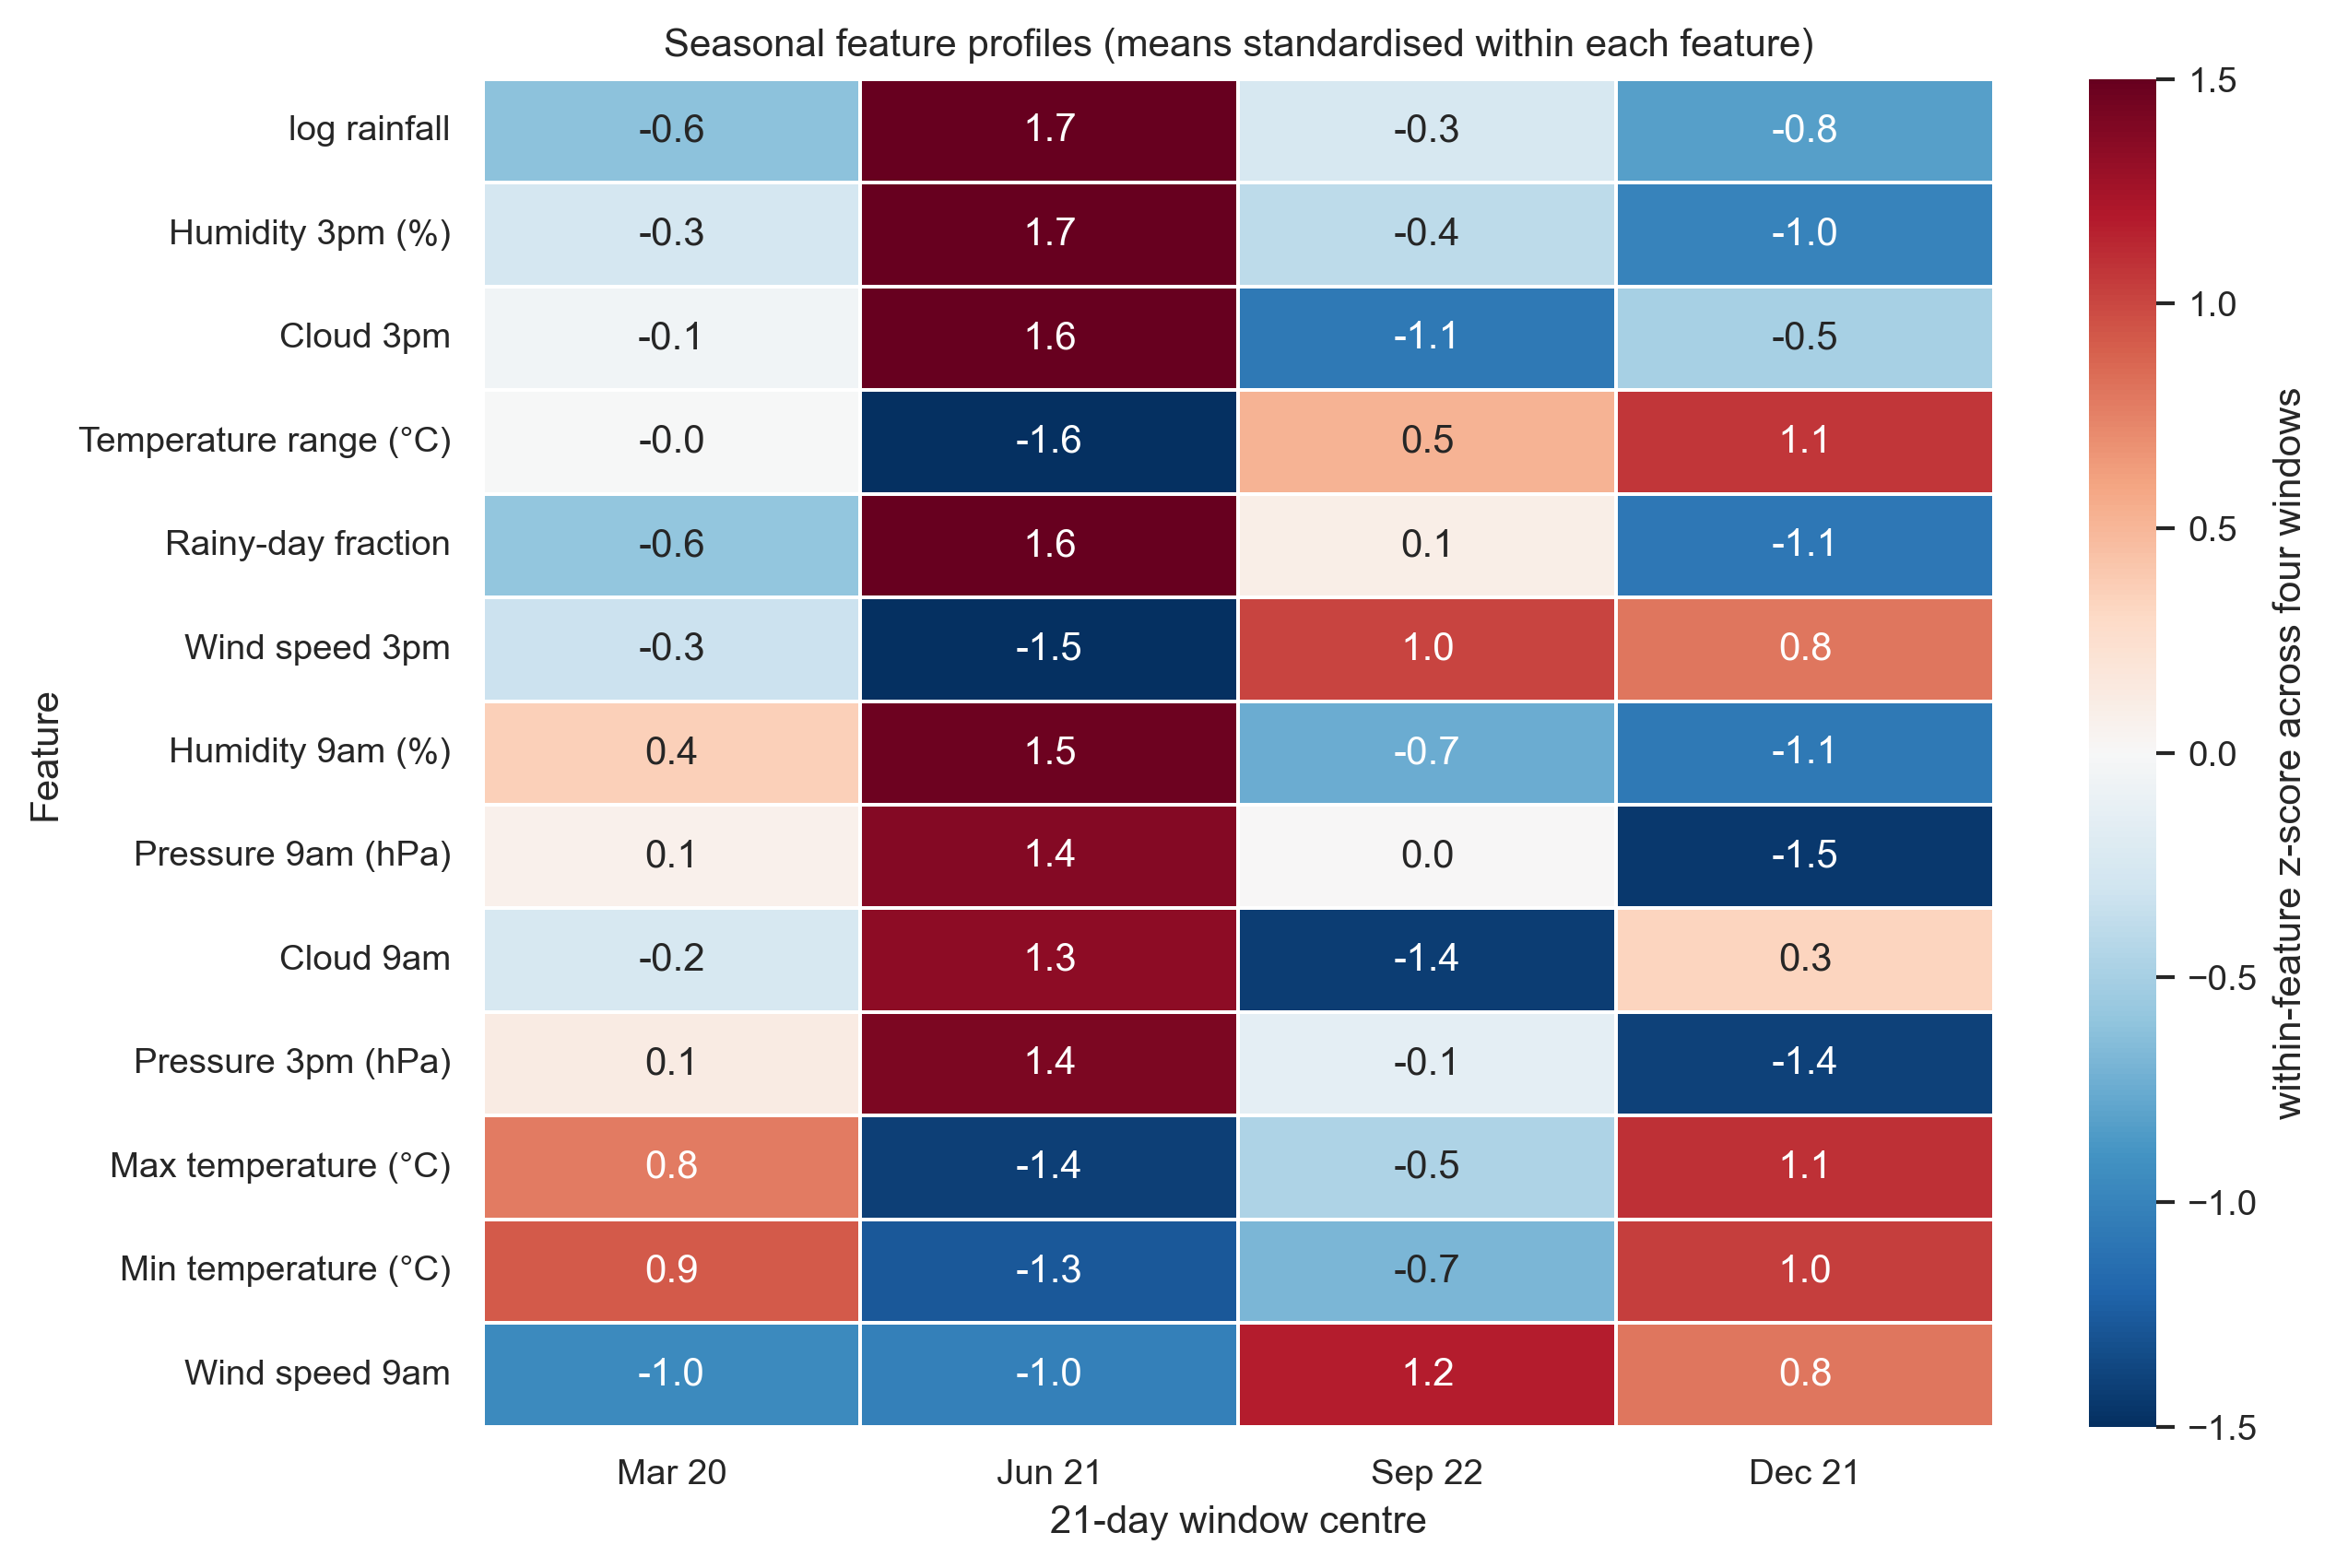
\includegraphics[width=0.95\linewidth]{p7_seasonal_feature_profile}
\caption{Seasonal feature profiles. Each row is standardised within that feature across the four windows, so pressure, temperature and rainfall do not share a misleading raw axis.}\label{fig:seasonfeatures}
\end{figure}

\subsection{Seasonal t-SNE and prediction}
The seasonal t-SNE uses median imputation and scaling on all station-year rows for visualization only. Its zone silhouette in the embedded space is \SeasonTsneSil{}. The figure is suggestive rather than inferential because a station contributes several related years; the prediction experiment below still holds out complete stations.

\begin{figure}[t]\centering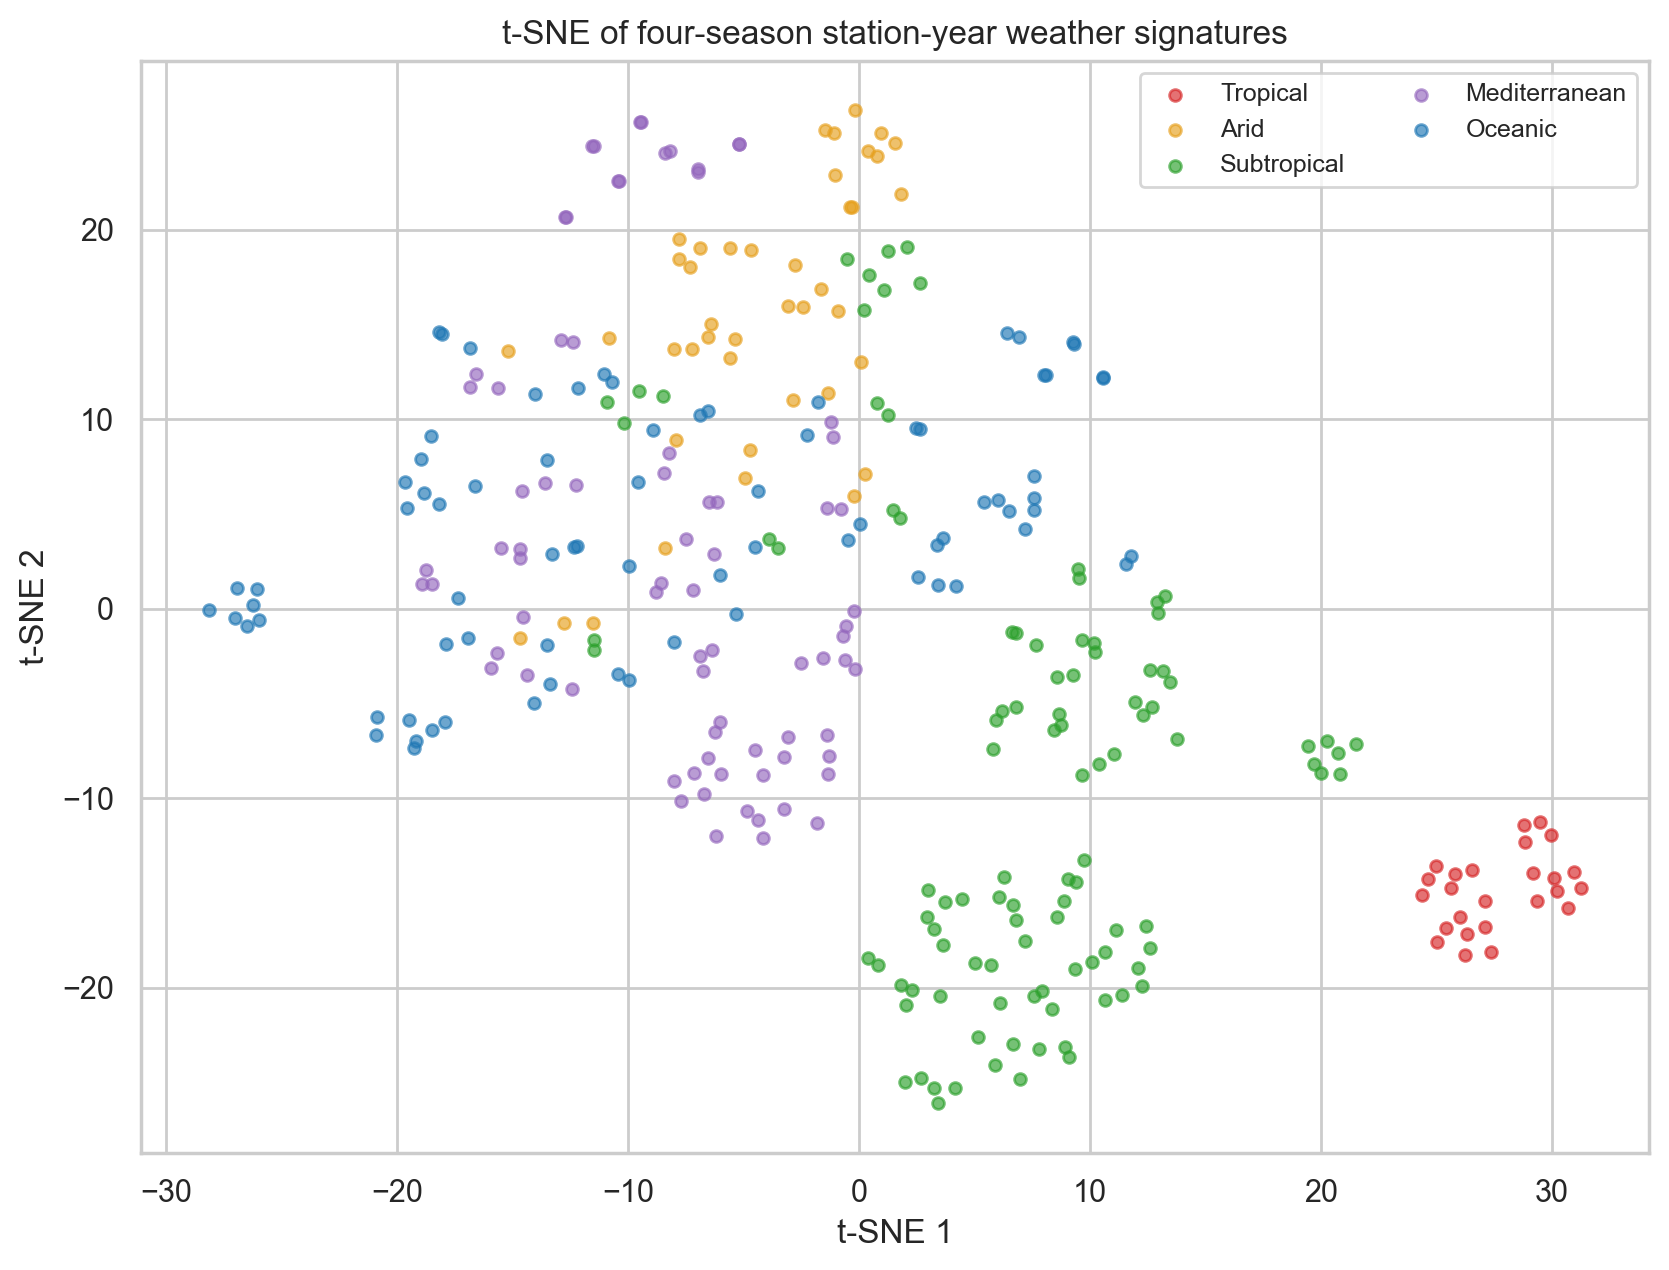
\includegraphics[width=0.92\linewidth]{p7_seasonal_tsne}
\caption{t-SNE of four-season station-year signatures. Repeated years from one station are retained for descriptive visualization; outer prediction remains station-disjoint.}\label{fig:seasontsne}
\end{figure}

The main supervised comparison uses four station-held-out folds and three reused partition seeds. LR, tuned DT, RF and tuned HGB are fitted within each training fold; tuning uses three station-disjoint inner folds. Seasonal LR reaches \SeasonLR{} macro-F1 and \SeasonLRAUC{} macro-AUC, while tuned HGB reaches \SeasonHGB{}. Across all 12 outer fold scores for LR, the mean is \SeasonFoldMean{} with SD \SeasonFoldSD{} and range \SeasonFoldMin{}--\SeasonFoldMax{}. A station-bootstrap interval conditional on the saved seed-42 predictions is \SeasonBootLow{}--\SeasonBootHigh{}; it excludes refitting and model-selection uncertainty. The simple model wins in this comparison because the seasonal representation makes the relevant contrasts more available to a linear decision rule; we do not interpret that as a universal advantage of LR.

\begin{table}[t]
\centering
\small
\setlength{\tabcolsep}{4pt}
\caption{Four-season station-year signature models. Every outer fold holds out complete stations.}\label{tab:season}
\begin{tabular}{lrrrrr}\toprule
Model & Primary F1 & Seed mean & Seed range & Station-bal. & AUC \\ \midrule
LR & 0.861 & 0.854 & 0.831--0.869 & 0.855 & 0.973 \\
DT-tuned & 0.684 & 0.669 & 0.643--0.684 & 0.682 & 0.844 \\
RF & 0.803 & 0.802 & 0.775--0.828 & 0.796 & 0.957 \\
HGB-tuned & 0.807 & 0.801 & 0.775--0.823 & 0.798 & 0.943 \\
\bottomrule
\end{tabular}
\end{table}
\begin{figure}[t]\centering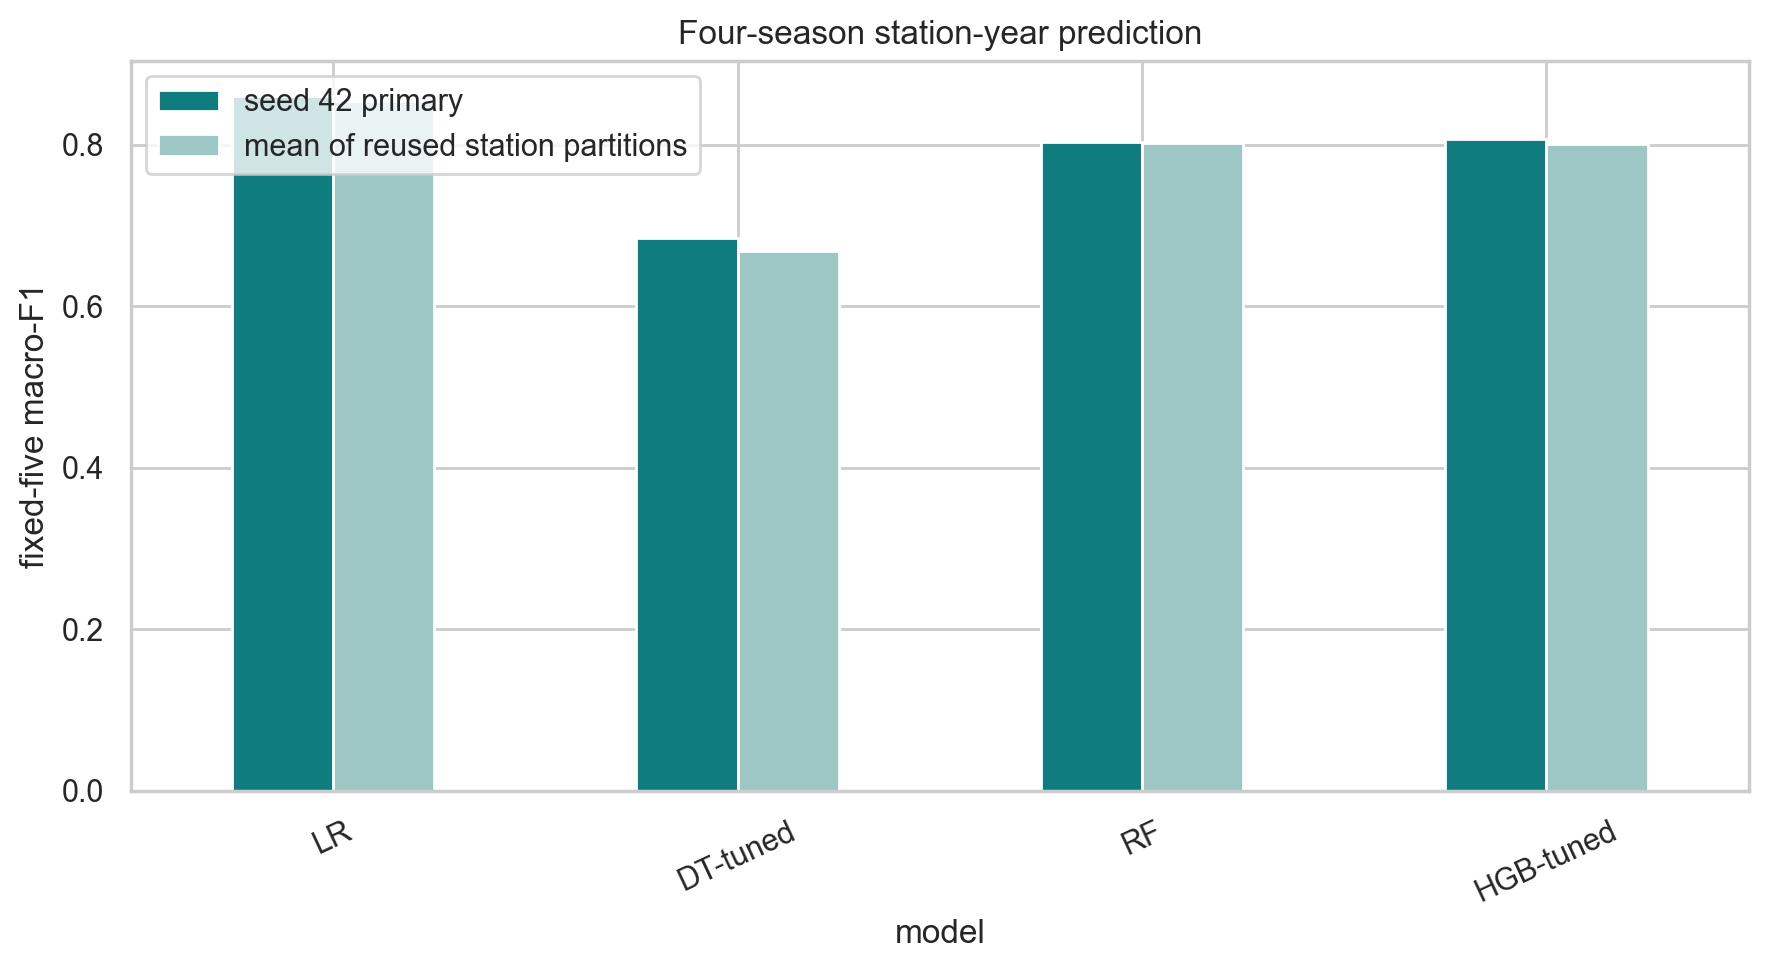
\includegraphics[width=\linewidth]{p7_seasonal_model_comparison}
\caption{Station-held-out seasonal model comparison. Bars show the designated seed-42 partition and the mean over three reused station partitions.}\label{fig:seasonmodels}
\end{figure}

The primary seasonal LR per-class scores are given below. Tropical is easy to recognise but has only 25 retained station-years; Arid and Oceanic remain the less stable groups.

\begin{table}[t]
\centering
\small
\setlength{\tabcolsep}{4pt}
\caption{Per-class precision, recall and F1 for the primary seasonal LR model.}\label{tab:class}
\begin{tabular}{lrrrr}\toprule
Zone & Prec. & Recall & F1 & Support \\ \midrule
Tropical & 1.000 & 1.000 & 1.000 & 25 \\
Arid & 0.696 & 0.762 & 0.727 & 42 \\
Subtropical & 0.923 & 0.906 & 0.914 & 106 \\
Mediterranean & 0.851 & 0.818 & 0.834 & 77 \\
Oceanic & 0.823 & 0.833 & 0.828 & 78 \\
\bottomrule
\end{tabular}
\end{table}

We then ask whether the seasonal gain is merely the result of showing the model four more rows. For every station-year we take the daily out-of-fold prediction nearest each window centre and vote across those four snapshots. Keeping the classifier family fixed, daily HGB reaches \MatchedDaily{} and seasonal HGB reaches \SeasonHGB{}, an increase of \SeasonGain{} (0.048 if the displayed rounded scores are subtracted). The corresponding LR comparison is \MatchedLR{} to \SeasonLR{}, an increase of \SeasonLRGain{}. We therefore compare within HGB and LR separately, rather than subtracting the seasonal LR score from the daily HGB score. The matched results support our mechanism: summaries across windows add information beyond four isolated weather snapshots, although they also change the observation unit and discard incomplete station-years.

\subsection{History and model sensitivity}
We also compare trailing means over 1, 3, 7, 14, 30, 90 and 365 days. Nested station-held-out selection gives LR \HistoryLR{} and HGB \HistoryHGB{} macro-F1. The best window differs by model and partition, so we do not claim that one history length is universally optimal. Polynomial LR reaches \DailyPoly{} on daily inputs and RF reaches \DailyRF{}. A 100-km exclusion-buffer stress test lowers fixed HGB to \SpatialHGB{} while also reducing the available training stations; this shows that transfer across the observed network is practically relevant, but it does not isolate a single causal source of the drop. Missingness policies, feature-selection scores, fold assignments and station errors are exported in \texttt{results/}.

\section{Limitations and conclusion}
Four seasonal windows are a defensible proxy for an annual weather pattern, but Köppen classes are built from longer climatological normals. We have only 48 labelled stations and four Tropical stations; years within a station are related; and the target comes from one manually matched raster annotation. The completeness filter has class-dependent coverage. External ARI helps us interpret unsupervised structure, but it is not a training target and does not prove that we recovered a physical climate boundary. Holding out stations supports transfer within this network, not unconditional accuracy at arbitrary Australian sites or claims about future climate change.

We began with a single day because that is what the dataset gives us most directly. The daily t-SNE and clusters showed why that view is limited: weather states are real and interpretable, but they cross climate boundaries. Monthly station profiles then showed the bridge we were looking for: weather similarity has both regional structure and cross-region recurrence. The four-window signature turns that idea into a supervised test. In this station network, it improves the daily vote within each classifier family and makes a simple LR the strongest tested model. Our conclusion is therefore about representation: temporal coverage carries more climate-label signal than one snapshot in this dataset. It is not a claim that four dates define climate everywhere.

\section*{Reproducibility}
The executed notebook contains all code, figures and explanatory text. The final run has 122 executed cells, 48 stations, \SeasonRows{} seasonal rows and run identifier \texttt{\RunID}. Python \PythonVersion{} and pinned dependencies are recorded in the requirements file. CSV exports, predictions, fold assignments and diagnostic tables are in \texttt{results/}; the notebook code hash and raw-data hashes are recorded in \texttt{run\_manifest.json} and \texttt{environment.json}. The raw weather data are unchanged.

\clearpage
\begin{thebibliography}{10}\small
\bibitem{kaggle} Kaggle user jsphyg. Rain in Australia, version 2. \url{https://www.kaggle.com/datasets/jsphyg/weather-dataset-rattle-package}.
\bibitem{bom} Bureau of Meteorology. Station list IDCJMC0014. The project includes the station crosswalk used for annotation.
\bibitem{kgc} Rubel et al. World maps of the Köppen--Geiger climate classification, reference period 1986--2010. \url{https://koeppen-geiger.vu-wien.ac.at/present.htm}.
\bibitem{sklearn} Pedregosa et al. Scikit-learn: Machine learning in Python. \emph{JMLR}, 12:2825--2830, 2011.
\bibitem{tsne} van der Maaten and Hinton. Visualizing data using t-SNE. \emph{JMLR}, 9:2579--2605, 2008.
\bibitem{ari} Hubert and Arabie. Comparing partitions. \emph{Journal of Classification}, 2:193--218, 1985.
\bibitem{rf} Breiman. Random forests. \emph{Machine Learning}, 45:5--32, 2001.
\bibitem{boost} Friedman. Greedy function approximation: a gradient boosting machine. \emph{Annals of Statistics}, 29:1189--1232, 2001.
\end{thebibliography}

\section*{Credit}
Group 7 members are QIAO, Xiaolong; MO, Zijun; WANG, Zhifei; and XIA, Youyue. Contribution percentages must be confirmed by the group before submission and should sum to 100\%; this report does not infer personal contributions from code or results. We used OpenAI Codex for coding support, debugging, experiment review, reproducibility checks and drafting or polishing explanatory text. Group members inspected the generated material, reran the notebook and checked the reported values against the executed outputs. The presentation also contains a decorative AI-generated illustration, which is not data or evidence. The activity log is in \texttt{AI\_LOG.md}.
\end{document}
